\documentclass[14pt]{beamer}
\setbeamertemplate{footline}[frame number]

\usepackage{appendixnumberbeamer}
\usepackage{xcolor}
\usepackage[official]{eurosym}
% Math packages
\usepackage{amsmath,amsfonts,amssymb,amsthm}
\usepackage{mathrsfs}
\usepackage{thmtools}
\usepackage{array}
\usepackage{cleveref}
\usepackage{stmaryrd}
\usepackage{mathpartir}


% Command control packages
\usepackage{ifthen}
\usepackage{ifpdf}

% Listings
\usepackage{listings}
\lstset{
  basicstyle=\ttfamily,
  columns=fullflexible,
  keepspaces=true,
  mathescape
}


% Tikz
\usepackage{tikz}

%%% Comments
% Comments
\newcommand\lau[1]{{\color{purple} \sf \footnotesize {LS: #1}}\\}
\newcommand\dominique[1]{{\color{purple} \sf \footnotesize {DD: #1}}\\}
\newcommand\lars[1]{{\color{purple} \sf \footnotesize {LB: #1}}\\}

%%% Math environments
\declaretheorem[numbered=yes,name=Lemma,qed=$\blacksquare$]{lemma}
\declaretheorem[numbered=yes,name=Theorem,qed=$\blacksquare$]{theorem}
\declaretheorem[numbered=yes,name=Definition,qed=$\blacksquare$]{definition}
\declaretheorem[numbered=yes,name=Specification,qed=$\blacksquare$]{specification}


%%% Math notation
\newcommand{\defeq}{\stackrel{\textit{\tiny{def}}}{=}}
\newcommand{\defbnf}{::=}
\newcommand{\sem}[1]{\left\llbracket #1 \right\rrbracket}
\newcommand{\ssem}[2][\Phi]{\sem{#2}_{\mathrm{src}}(#1)}
\newcommand{\tsem}[2][\Phi]{\sem{#2}_{\mathrm{trg}}(#1)}
\newcommand{\dom}{\mathrm{dom}}
\newcommand{\powerset}[1]{\mathcal{P}(#1)}

\newcommand{\npair}[2][n]{\left(#1,#2\right)}

\newcommand{\nsubeq}[1][n]{\overset{#1}{\subseteq}}
\newcommand{\nsupeq}[1][n]{\overset{#1}{\supseteq}}
\newcommand{\nequal}[1][n]{\overset{#1}{=}}

% Function arrows
\newcommand{\fun}{\rightarrow}
\newcommand{\parfun}{\rightharpoonup}
\newcommand{\monnefun}{\xrightarrow{\textit{\tiny{mon, ne}}}}



% Text
\newcommand{\tand}{\text{ and }}
\newcommand{\tor}{\text{ or }}
\newcommand{\totherwise}{\text{otherwise }}

% Equivalences
\newcommand{\sconeq}{\mathrel{\src{\approx_{\mathrm{ctx}}}}}
\newcommand{\tconeq}{\mathrel{\approx_{\mathrm{ctx}}}}

%%% Logical Relation notation
\newcommand{\typesetlr}[1]{\mathcal{#1}}
\newcommand{\lre}{\typesetlr{E}}
\newcommand{\lrexj}{\typesetlr{E}_{\var{xjmp}}}
\newcommand{\lrk}{\typesetlr{K}}
\newcommand{\lrr}{\typesetlr{R}}
\newcommand{\lro}{\typesetlr{O}}
\newcommand{\lrv}{\typesetlr{V}}
\newcommand{\lrp}{\typesetlr{P}}
\newcommand{\lrm}{\typesetlr{M}}

\newcommand{\stpair}[3][]{
\ifthenelse{\equal{#1}{}}
{\left(\src{#2_S},#3_T\right)}
{\left(\src{#2},#3\right)}}


\newcommand{\memSat}[3][n]{#2 :_{#1}#3}

\newcommand{\World}{\mathrm{World}}
\newcommand{\RegionName}{\mathrm{RegionName}}
\newcommand{\Region}{\mathrm{Region}}
\newcommand{\spatial}{\mathrm{spatial}}
\newcommand{\spatialo}{\mathrm{spatial\_owned}}
\newcommand{\pure}{\mathrm{pure}}
\newcommand{\revoked}{\mathrm{revoked}}
\newcommand{\State}{\mathrm{State}}
\newcommand{\Rels}{\mathrm{Rels}}
\newcommand{\UPred}[1]{\mathrm(#1)}

\newcommand{\future}{\sqsupseteq}
\newcommand{\pub}{\mathrm{pub}}
\newcommand{\privft}{\future^{\priv}}
\newcommand{\pubft}{\future^{\pub}}
\newcommand{\monprivnefun}{\xrightarrow[\text{\tiny{$\privft$}}]{\textit{\tiny{mon, ne}}}}
\newcommand{\monpubnefun}{\xrightarrow[\text{\tiny{$\pubft$}}]{\textit{\tiny{mon, ne}}}}

%%% Regions
\newcommand{\stdreg}[2]{\iota^{\mathrm{std},#2}_{#1}}
\newcommand{\stareg}[2][\stpair{\ms}{\ms}]{\iota^{\mathrm{sta},#2}_{#1}}
\newcommand{\spa}{\mathrm{s}}
\newcommand{\spao}{\mathrm{so}}
\newcommand{\pur}{\mathrm{p}}

%%% Instruction formatting
\newcommand{\sourcecolortext}{blue}
\newcommand{\sourcecolor}{\color{blue}}
\newcommand{\src}[1]{{\sourcecolor #1}}
\newcommand{\targetcolortext}{black}
\newcommand{\targetcolor}[1]{\color{black}}
\newcommand{\trg}[1]{{\targetcolor{} #1}}

\newcommand{\zinstr}[1]{\texttt{#1}}
\newcommand{\oneinstr}[2]{
  \ifthenelse{\equal{#2}{}}
  {\zinstr{#1}}
  {\zinstr{#1} \; #2}
}
\newcommand{\twoinstr}[3]{
  \ifthenelse{\equal{#2#3}{}}
  {\zinstr{#1}}
  {\zinstr{#1} \; #2 \; #3}
}
\newcommand{\threeinstr}[4]{
  \ifthenelse{\equal{#2#3#4}{}}
  {\zinstr{#1}}
  {\zinstr{#1} \; #2 \; #3 \; #4}
}

\newcommand{\fourinstr}[5]{
  \ifthenelse{\equal{#2#3#4#5}{}}
  {\zinstr{#1}}
  {\zinstr{#1} \; #2 \; #3 \; #4 \; #5}
}


%%% Source language
% No arguments
\newcommand{\sfail}{\zinstr{\src{fail}}}
\newcommand{\shalt}{\zinstr{\src{halt}}}
\newcommand{\sreturn}{\zinstr{\src{return}}}

% One argument
\newcommand{\sjmp}[1]{\oneinstr{\src{jmp}}{#1}}
\newcommand{\spush}[1]{\oneinstr{\src{push}}{#1}}
\newcommand{\spop}[1]{\oneinstr{\src{pop}}{#1}}

% Two arguments
\newcommand{\sjnz}[2]{\twoinstr{\src{jnz}}{#1}{#2}}
\newcommand{\sisptr}[2]{\twoinstr{\src{gettype}}{#1}{#2}}
\newcommand{\sgeta}[2]{\twoinstr{\src{geta}}{#1}{#2}}
\newcommand{\sgetb}[2]{\twoinstr{\src{getb}}{#1}{#2}}
\newcommand{\sgete}[2]{\twoinstr{\src{gete}}{#1}{#2}}
\newcommand{\sgetp}[2]{\twoinstr{\src{getp}}{#1}{#2}}
%\newcommand{\sgetloc}[2]{\twoinstr{\src{getloc}}{#1}{#2}}
\newcommand{\sgetlin}[2]{\twoinstr{\src{get}}{#1}{#2}}
\newcommand{\smove}[2]{\twoinstr{\src{move}}{#1}{#2}}
\newcommand{\sstore}[2]{\twoinstr{\src{store}}{#1}{#2}}
\newcommand{\sload}[2]{\twoinstr{\src{load}}{#1}{#2}}
\newcommand{\scca}[2]{\twoinstr{\src{cca}}{#1}{#2}}
\newcommand{\ssload}[2]{\twoinstr{\src{sload}}{#1}{#2}}
\newcommand{\sxjmp}[2]{\twoinstr{\src{xjmp}}{#1}{#2}}
\newcommand{\ssetatob}[2]{\twoinstr{\src{seta2b}}{#1}{#2}}
% scall - special two instruction
\newcommand{\scall}[4][]{  
\ifthenelse{\equal{#3#4}{}}
  {\ensuremath{\zinstr{\src{call}}_{#1}^{#2}}}
  {\ensuremath{\zinstr{\src{call}}_{#1}^{#2} \; #3 \; #4}}
}


% Three arguments
\newcommand{\srestrict}[3]{\threeinstr{\src{restrict}}{#1}{#2}{#3}}
\newcommand{\slt}[3]{\threeinstr{\src{lt}}{#1}{#2}{#3}}
\newcommand{\splus}[3]{\threeinstr{\src{plus}}{#1}{#2}{#3}}
\newcommand{\sminus}[3]{\threeinstr{\src{minus}}{#1}{#2}{#3}}
\newcommand{\scseal}[3]{\threeinstr{\src{cseal}}{#1}{#2}{#3}}
\newcommand{\ssplice}[3]{\threeinstr{\src{splice}}{#1}{#2}{#3}}


% Four arguments
%\newcommand{\ssubseg}[4]{\fourinstr{\src{subseg}}{#1}{#2}{#3}{#4}}
\newcommand{\ssplit}[4]{\fourinstr{\src{split}}{#1}{#2}{#3}{#4}}

%%% Target language
% No arguments
\newcommand{\tfail}{\zinstr{\trg{fail}}}
\newcommand{\thalt}{\zinstr{\trg{halt}}}

% One argument
\newcommand{\tjmp}[1]{\oneinstr{\trg{jmp}}{#1}}

% Two arguments
\newcommand{\tjnz}[2]{\twoinstr{\trg{jnz}}{#1}{#2}}
\newcommand{\tisptr}[2]{\twoinstr{\trg{gettype}}{#1}{#2}}
\newcommand{\tgeta}[2]{\twoinstr{\trg{geta}}{#1}{#2}}
\newcommand{\tgetb}[2]{\twoinstr{\trg{getb}}{#1}{#2}}
\newcommand{\tgete}[2]{\twoinstr{\trg{gete}}{#1}{#2}}
\newcommand{\tgetp}[2]{\twoinstr{\trg{getp}}{#1}{#2}}
%\newcommand{\tgetloc}[2]{\twoinstr{\trg{getloc}}{#1}{#2}}
\newcommand{\tgetlin}[2]{\twoinstr{\trg{getl}}{#1}{#2}}
\newcommand{\tmove}[2]{\twoinstr{\trg{move}}{#1}{#2}}
\newcommand{\tstore}[2]{\twoinstr{\trg{store}}{#1}{#2}}
\newcommand{\tload}[2]{\twoinstr{\trg{load}}{#1}{#2}}
\newcommand{\tcca}[2]{\twoinstr{\trg{cca}}{#1}{#2}}
\newcommand{\txjmp}[2]{\twoinstr{\trg{xjmp}}{#1}{#2}}
\newcommand{\tsetatob}[2]{\twoinstr{\trg{seta2b}}{#1}{#2}}

% Three arguments
\newcommand{\tsplice}[3]{\threeinstr{\trg{splice}}{#1}{#2}{#3}}
\newcommand{\trestrict}[3]{\threeinstr{\trg{restrict}}{#1}{#2}{#3}}
\newcommand{\tlt}[3]{\threeinstr{\trg{lt}}{#1}{#2}{#3}}
\newcommand{\tplus}[3]{\threeinstr{\trg{plus}}{#1}{#2}{#3}}
\newcommand{\tminus}[3]{\threeinstr{\trg{minus}}{#1}{#2}{#3}}
\newcommand{\tcseal}[3]{\threeinstr{\trg{cseal}}{#1}{#2}{#3}}

% Four arguments
%\newcommand{\tsubseg}[4]{\fourinstr{\trg{subseg}}{#1}{#2}{#3}{#4}}
\newcommand{\tsplit}[4]{\fourinstr{\trg{split}}{#1}{#2}{#3}{#4}}

%%% Domains
\newcommand{\plaindom}[1]{\mathrm{#1}}

\newcommand{\nats}{\mathbb{N}}
\newcommand{\ints}{\mathbb{Z}}

%%% Updates
\newcommand{\update}[2]{[#1 \mapsto #2]}
\newcommand{\updReg}[2]{\update{\reg.#1}{#2}}
\newcommand{\updPc}[1]{\Phi\updReg{\pcreg}{#1}}

%%% Source dom
\newcommand{\shareddom}[1]{\mathrm{#1}}
\newcommand{\RegName}{\shareddom{RegisterName}}
\newcommand{\Addr}{\shareddom{Addr}}
\newcommand{\Seal}{\shareddom{Seal}}
\newcommand{\Perm}{\shareddom{Perm}}
\newcommand{\Caps}{\shareddom{Cap}}
\newcommand{\SealableCaps}{\shareddom{SealableCap}}
\newcommand{\Word}{\shareddom{Word}}
\newcommand{\Instr}{\shareddom{Instr}}
\newcommand{\Mem}{\shareddom{Memory}}
\newcommand{\Reg}{\shareddom{RegisterFile}}
\newcommand{\Stk}{\shareddom{Stack}}
\newcommand{\Conf}{\shareddom{Conf}}
\newcommand{\ExecConf}{\shareddom{ExecConf}}
%\newcommand{\Global}{\shareddom{Global}}
\newcommand{\Linear}{\shareddom{Linear}}
\newcommand{\MemSeg}{\shareddom{MemorySegment}}
\newcommand{\StkFrame}{\shareddom{StackFrame}}
\newcommand{\Stack}{\shareddom{Stack}}

\newcommand{\scbnf}{\shareddom{sc}}
\newcommand{\cbnf}{\shareddom{c}}
\newcommand{\permbnf}{\shareddom{perm}}
\newcommand{\addrbnf}{\shareddom{a}}
\newcommand{\basebnf}{\shareddom{base}}
\newcommand{\aendbnf}{\shareddom{end}}
\newcommand{\rbnf}{\shareddom{r}}
%\newcommand{\glbnf}{\shareddom{gl}}
\newcommand{\linbnf}{\shareddom{l}}
\newcommand{\sealbasebnf}{\sigma_\shareddom{base}}
\newcommand{\sealendbnf}{\sigma_\shareddom{end}}

\newcommand{\sstk}{\shareddom{stk}}
\newcommand{\smsstk}{\shareddom{ms_{stk}}}
\newcommand{\sstkframe}{\shareddom{frame}}
\newcommand{\sopc}{\shareddom{opc}}
\newcommand{\sastk}{\shareddom{a_{stk}}}
\newcommand{\perm}{\var{perm}}
%\newcommand{\gl}{\var{g}}
\newcommand{\lin}{\var{l}}
\newcommand{\base}{\shareddom{base}}
\newcommand{\aend}{\shareddom{end}}
\newcommand{\addr}{\shareddom{a}}
\newcommand{\scap}{\shareddom{c}}
\newcommand{\sms}{\shareddom{ms}}

\newcommand{\stkptr}[1]{\mathrm{stack\text{-}ptr}(#1)}
\newcommand{\retptr}{\mathrm{ret\text{-}ptr}}
\newcommand{\retptrd}{\mathrm{ret\text{-}ptr\text{-}data}}
\newcommand{\retptrc}{\mathrm{ret\text{-}ptr\text{-}code}}

\newcommand{\seal}[1]{\shareddom{seal}(#1)}
\newcommand{\sealed}[1]{\shareddom{sealed}(#1)}

\newcommand{\failed}{\mathrm{failed}}
% DOMI: defining a macro named ``undefined'' breaks many latex packages.
%       (this is just another way that LaTeX is broken as a programming language)
% \newcommand{\undefined}{\mathrm{undefined}}
\newcommand{\tundefined}{\mathrm{undefined}}
\newcommand{\halted}{\mathrm{halted}}

%%% Target domain
\newcommand{\targetdom}[1]{\mathrm{#1}}
\newcommand{\tRegName}{\targetdom{RegisterName}}

%%% Programs and contexts
\newcommand{\program}{\mathscr{P}}
\newcommand{\context}{\mathscr{C}}

\newcommand{\plug}[2]{#1[#2]}

%%% Operational semantics
\newcommand{\step}{\rightarrow}
\newcommand{\nstep}[1][n]{\step_{#1}}
\newcommand{\steps}{\step^*}
\newcommand{\diverge}{{\Uparrow}}
\newcommand{\term}[1][-]{{\Downarrow_{#1}}}

%%% Variables
\newcommand{\var}[1]{\mathit{#1}}
\newcommand{\rn}{\var{rn}}
\newcommand{\reg}{\var{reg}}
\newcommand{\mem}{\var{mem}}
\newcommand{\ms}{\var{ms}}
\newcommand{\pc}{\var{pc}}
\newcommand{\stk}{\var{stk}}
\newcommand{\link}{\var{link}}
\newcommand{\stkf}{\stk_{\var{frame}}}
\newcommand{\ret}{\var{ret}}
\newcommand{\data}{\var{data}}
\newcommand{\code}{\var{code}}
\newcommand{\priv}{\var{priv}}
\newcommand{\opc}{\var{opc}}
\newcommand{\odata}{\var{odata}}
\newcommand{\vsc}{\var{sc}}
\newcommand{\cb}{\vsc}
\newcommand{\baddr}{\var{b}}
\newcommand{\eaddr}{\var{e}}
\newcommand{\aaddr}{\var{a}}
\newcommand{\stdrng}{[\baddr,\eaddr]}

%%% Constants
\newcommand{\constant}[1]{\mathrm{#1}}
\newcommand{\calllen}{\constant{call\_len}}
\newcommand{\stkb}{\constant{stk\_base}}

%%% Named registers
\newcommand{\pcreg}{\mathrm{pc}}
\newcommand{\rstk}{\mathrm{r}_\mathrm{stk}}
\newcommand{\rO}{\mathrm{r}_\mathrm{ret}}
\newcommand{\rret}{\rO}
\newcommand{\rretc}{\mathrm{r}_\mathrm{ret code}}
\newcommand{\rretd}{\mathrm{r}_\mathrm{ret data}}
\newcommand{\rdata}{\mathrm{r}_\mathrm{data}}
\newcommand{\rtmp}[1]{\mathrm{r}_\mathrm{t#1}}



%%% locality
%\newcommand{\plainlocality}[1]{\mathrm{#1}}
%\newcommand{\glob}{\plainlocality{global}}
%\newcommand{\local}{\plainlocality{local}}

%%% linearity
\newcommand{\plainlinearity}[1]{\mathrm{#1}}
\newcommand{\linear}{\plainlinearity{linear}}
\newcommand{\normal}{\plainlinearity{normal}}


%%% Permissions
\newcommand{\plainperm}[1]{\textsc{#1}}
%\newcommand{\rwlx}{\plainperm{rwlx}}
\newcommand{\rwx}{\plainperm{rwx}}
\newcommand{\rx}{\plainperm{rx}}
%\newcommand{\rwlxo}{\plainperm{rwlxo}}
%\newcommand{\rwlo}{\plainperm{rwlo}}
%\newcommand{\rwl}{\plainperm{rwl}}
%\newcommand{\rwxo}{\plainperm{rwxo}}
%\newcommand{\rwo}{\plainperm{rwo}}
\newcommand{\rw}{\plainperm{rw}}
%\newcommand{\rxo}{\plainperm{rxo}}
\newcommand{\readonly}{\plainperm{r}}
\newcommand{\ro}{\readonly}
\newcommand{\noperm}{\plainperm{0}}
%\newcommand{\nopermo}{\plainperm{0o}}
%\newcommand{\enter}{\plainperm{e}}
%\newcommand{\entero}{\plainperm{eo}}

%%% Braces
\newcommand{\comp}[1]{[#1]}

%%% Functions
\newcommand{\plainfun}[2]{
  \ifthenelse{\equal{#2}{}}
  {\mathit{#1}}
  {\mathit{#1}(#2)}
}

%\newcommand{\isLoc}[1]{\plainfun{isLocal}{#1}}
%\newcommand{\nonLoc}[1]{\plainfun{nonLocal}{#1}}
%\newcommand{\opaquePerm}[1]{\plainfun{opaquePerm}{#1}}
%\newcommand{\updPcPerm}[1]{\plainfun{updatePcPerm}{#1}}
%\newcommand{\writeLocalAllowed}[1]{\plainfun{writeLocalAllowed}{#1}}
\newcommand{\addressable}[1]{\plainfun{addressable}{#1}}
\newcommand{\callCond}[1]{\plainfun{callCondition}{#1}}
\newcommand{\decInstr}[1]{\plainfun{decodeInstruction}{#1}}
\newcommand{\decPerm}[1]{\plainfun{decodePerm}{#1}}
\newcommand{\encInstr}[1]{\plainfun{encodeInstruction}{#1}}
\newcommand{\encPerm}[1]{\plainfun{encocePerm}{#1}}
\newcommand{\encLin}[1]{\plainfun{encoceLin}{#1}}
\newcommand{\encType}[1]{\plainfun{encodeType}{#1}}
\newcommand{\exec}[1]{\plainfun{executable}{#1}}
\newcommand{\execCond}[1]{\plainfun{executeCondition}{#1}}
\newcommand{\isLinear}[1]{\plainfun{isLinear}{#1}}
\newcommand{\linCons}[1]{\plainfun{linearityConstraint}{#1}}
\newcommand{\noRetStkMs}[1]{\plainfun{noRetStk_{ms}}{#1}}
\newcommand{\noRetStkReg}[1]{\plainfun{noRetStk_{reg}}{#1}}
\newcommand{\nonExec}[1]{\plainfun{nonExecutable}{#1}}
\newcommand{\nonLinear}[1]{\plainfun{nonLinear}{#1}}
\newcommand{\nonZero}[1]{\plainfun{nonZero}{#1}}
\newcommand{\range}[1]{\plainfun{range}{#1}}
\newcommand{\readAllowed}[1]{\plainfun{readAllowed}{#1}}
\newcommand{\readCond}[1]{\plainfun{readCondition}{#1}}
\newcommand{\writeCond}[1]{\plainfun{writeCondition}{#1}}
\newcommand{\sealAss}[1]{\plainfun{sealAssignment}{#1}}
\newcommand{\updPcAddr}[1]{\plainfun{updatePc}{#1}}
\newcommand{\withinBounds}[1]{\plainfun{withinBounds}{#1}}
\newcommand{\writeAllowed}[1]{\plainfun{writeAllowed}{#1}}
\newcommand{\xjumpResult}[3]{\plainfun{xjumpResult}{#1,#2,#3}}

\usepackage{ifthen}
\usepackage{pgf}
\usepackage{ulem}
\usepackage{tikz}
\usepackage{tikzpeople}
\usetikzlibrary{backgrounds}
\usetikzlibrary{fit}
\usetikzlibrary{calc}
\usetikzlibrary{positioning}
\usetikzlibrary{patterns}
\usetikzlibrary{decorations.pathreplacing}
\usetikzlibrary{arrows,shapes}
\usepackage{amssymb}

\newcommand{\sealsymb}[1]{
  \draw #1 node  {\footnotesize\faLock};
}

\newcommand{\sealsymbalt}[2][]{
  \draw #2 node {\footnotesize\faLock};
  \draw #2 node[yshift=-1.3pt,scale=0.8]  {\tiny\textcolor{white}{#1}};
}

\newcommand{\regfile}{
      \draw (17.5,5.5) node {register file};
    \begin{scope}
      \clip (16.9,1.1) rectangle (18.1,5.1);
      \foreach \x in {1,2,...,4}
      {
        \draw[fill=white] (17,\x) rectangle (18,\x+1) node[pos=.5,color=mygreen] {};
      };
    \end{scope}
    \coordinate (r1) at (17.5,4.5) {};
    \node[anchor=west] at (18.1,4.5) {$r_{\mathit{stk}}$};
    \coordinate (r2) at (17.5,3.5) {};
    \node[anchor=west] at (18.1,3.5) {$r_2$};
    \coordinate (r3) at (17.5,2.5) {};
    \node[anchor=west] at (18.1,2.5) {$r_3$};
}

% Active adversary
\newcommand{\actadv}[4][]{
  \ifthenelse{\equal{#1}{}}{
    \draw[fill=white] #2 rectangle #3 node[pos=.5] {};
    \draw ($#2 + (3,1.5)$) node[devil,mirrored,minimum size=0.9cm] {};
    \draw[fill=white, fill opacity=0.5] #2 rectangle #3 node[pos=.5] {};
    \draw #2 rectangle #3 node[pos=.5] {\scriptsize #4};
  }{
    \onlyenv<#1>
    \draw[fill=white] #2 rectangle #3 node[pos=.5] {};
    \draw ($#2 + (3,1.5)$) node[devil,mirrored,minimum size=0.9cm] {};
    \draw[fill=white, fill opacity=0.5] #2 rectangle #3 node[pos=.5] {};
    \draw #2 rectangle #3 node[pos=.5] {\scriptsize #4};
    \endonlyenv
  }
}

% Inactive adversary
\newcommand{\inactadv}[4][]{
  \ifthenelse{\equal{#1}{}}{
    \draw[fill=white] #2 rectangle #3 node[pos=.5] {};
    \draw ($#2 + (3,1.5)$) node[devil,mirrored,minimum size=0.9cm] {};
    \draw[fill=white, fill opacity=0.4] #2 rectangle #3 node[pos=.5] {};
    \draw[fill=gray, fill opacity=0.5] #2 rectangle #3 node[pos=.5] {};
    \draw #2 rectangle #3 node[pos=.5] {\scriptsize #4};
  }{
    \onlyenv<#1>
    \draw[fill=white] #2 rectangle #3 node[pos=.5] {};
    \draw ($#2 + (3,1.5)$) node[devil,mirrored,minimum size=0.9cm] {};
    \draw[fill=white, fill opacity=0.4] #2 rectangle #3 node[pos=.5] {};
    \draw[fill=gray, fill opacity=0.5] #2 rectangle #3 node[pos=.5] {};
    \draw #2 rectangle #3 node[pos=.5] {\scriptsize #4};
    \endonlyenv
  }
}

% Active stack frame
\newcommand{\actsf}[4][]{
  \ifthenelse{\equal{#1}{}}{
    \draw[fill=white] #2 rectangle #3 node[pos=.5] {\scriptsize #4};
  }{
   \draw<#1>[fill=white] #2 rectangle #3 node[pos=.5] {#4};
 }
}

% Inactive stack frame
\newcommand{\inactsf}[4][]{
  \ifthenelse{\equal{#1}{}}{
    \draw[fill=white] #2 rectangle #3 node[pos=.5] {};
    \draw[fill=gray, fill opacity=0.5] #2 rectangle #3 node[pos=.5] {};
    \draw #2 rectangle #3 node[pos=.5] {\scriptsize #4};
  }{
    \draw<#1>[fill=white] #2 rectangle #3 node[pos=.5] {};
    \draw<#1>[fill=gray, fill opacity=0.5] #2 rectangle #3 node[pos=.5] {};
    \draw<#1> #2 rectangle #3 node[pos=.5] {\scriptsize #4};
  }
}

\newcommand{\capbrace}[3][sp1]{
  \draw [decorate,decoration={brace,amplitude=8pt,mirror,raise=4pt},yshift=0pt]
  #2 -- #3 node[draw=black] (#1) [black,midway,xshift=0.8cm] {};
}

\newcommand{\stdstackstart}{
  \scope
    \clip (-.1,-.1) rectangle (6.1,15.1);
    \fill[fill=white] (0,0) rectangle (6,15);
    \draw (0,0) -- (0,15);
    \draw (6,0) -- (6,15);
    \draw[fill=gray!50] (0,-.5) rectangle (6,2.5) node[pos=.5] {\scriptsize lower stack frames...};
  \endscope
  % \draw[->] (-2,0) -- node[midway,sloped,above] {stack grows upward} (-2,15);
  \draw (-1.5,0) node {};
  \draw (-1.5,15) node {};
}


% stolen from https://tex.stackexchange.com/questions/14225/is-there-the-easiest-way-to-toggle-show-hide-navigational-grids-in-tikz/14230
\makeatletter
\newif\if@showgrid@grid
\newif\if@showgrid@left
\newif\if@showgrid@right
\newif\if@showgrid@below
\newif\if@showgrid@above
\tikzset{%
    every show grid/.style={},
    show grid/.style={execute at end picture={\@showgrid{grid=true,#1}}},%
    show grid/.default={true},
    show grid/.cd,
    labels/.style={font={\sffamily\small},help lines},
    xlabels/.style={},
    ylabels/.style={},
    keep bb/.code={\useasboundingbox (current bounding box.south west) rectangle (current bounding box.north west);},
    true/.style={left,below},
    false/.style={left=false,right=false,above=false,below=false,grid=false},
    none/.style={left=false,right=false,above=false,below=false},
    all/.style={left=true,right=true,above=true,below=true},
    grid/.is if=@showgrid@grid,
    left/.is if=@showgrid@left,
    right/.is if=@showgrid@right,
    below/.is if=@showgrid@below,
    above/.is if=@showgrid@above,
    false,
}

\def\@showgrid#1{%
    \begin{scope}[every show grid,show grid/.cd,#1]
    \if@showgrid@grid
    \begin{pgfonlayer}{background}
    \draw [help lines]
        (current bounding box.south west) grid
        (current bounding box.north east);
%
    \pgfpointxy{1}{1}%
    \edef\xs{\the\pgf@x}%
    \edef\ys{\the\pgf@y}%
    \pgfpointanchor{current bounding box}{south west}
    \edef\xa{\the\pgf@x}%
    \edef\ya{\the\pgf@y}%
    \pgfpointanchor{current bounding box}{north east}
    \edef\xb{\the\pgf@x}%
    \edef\yb{\the\pgf@y}%
    \pgfmathtruncatemacro\xbeg{ceil(\xa/\xs)}
    \pgfmathtruncatemacro\xend{floor(\xb/\xs)}
    \if@showgrid@below
    \foreach \X in {\xbeg,...,\xend} {
        \node [below,show grid/labels,show grid/xlabels] at (\X,\ya) {\X};
    }
    \fi
    \if@showgrid@above
    \foreach \X in {\xbeg,...,\xend} {
        \node [above,show grid/labels,show grid/xlabels] at (\X,\yb) {\X};
    }
    \fi
    \pgfmathtruncatemacro\ybeg{ceil(\ya/\ys)}
    \pgfmathtruncatemacro\yend{floor(\yb/\ys)}
    \if@showgrid@left
    \foreach \Y in {\ybeg,...,\yend} {
        \node [left,show grid/labels,show grid/ylabels] at (\xa,\Y) {\Y};
    }
    \fi
    \if@showgrid@right
    \foreach \Y in {\ybeg,...,\yend} {
        \node [right,show grid/labels,show grid/ylabels] at (\xb,\Y) {\Y};
    }
    \fi
    \end{pgfonlayer}
    \fi
    \end{scope}
}
\makeatother


\usepackage{pgfpages}
\setbeameroption{hide notes}
%\setbeameroption{show notes on second screen=right}
\usepackage{soul} 

\usepackage[numbers,square]{natbib}
\usepackage{bibentry}
\nobibliography*
\bibliographystyle{plain}

\definecolor{myred}{RGB}{192,58,45}
\definecolor{mypurple}{RGB}{180,52,202}
\definecolor{myblue}{RGB}{51,51,179}
\definecolor{mylblue}{RGB}{52,178,204}
\definecolor{mygreen}{RGB}{66,192,103}
\usepackage{tikzsymbols}

\usetikzlibrary{positioning}
\usetikzlibrary{fit}
\usetikzlibrary{decorations.pathreplacing}
\usetikzlibrary{calc}
\usetikzlibrary{arrows,shapes}

\tikzset{
    invisible/.style={opacity=0,text opacity=0},
    visible on/.style={alt=#1{}{invisible}},
    alt/.code args={<#1>#2#3}{%
      \alt<#1>{\pgfkeysalso{#2}}{\pgfkeysalso{#3}} 
    },
    beameralert/.style={alt=<#1>{fill=red!30,rounded corners}{},anchor=base},
    BeamerAlert/.style={alt=#1{fill=red!30,rounded corners}{},anchor=base}
}
\tikzset{capa/.style={decoration={markings,mark=at position 0 with %
      {\fill[black] circle(1.5pt);}}}}


\def\rotatechar#1{\reflectbox{#1}}
\newcommand{\capchar}{\euro{}}

\usepackage{graphicx}
\usepackage{dashrule}

\renewcommand{\ttdefault}{pcr}
\lstset{
  basicstyle=\ttfamily,
  columns=fullflexible,
  keepspaces=true,
  mathescape=true,
  literate={\$}{\$}{1},
  keywordstyle=\color{mylblue},
  tabsize=2
}

\lstdefinelanguage
   [x64]{Assembler}     % add a "x64" dialect of Assembler
   [x86masm]{Assembler} % based on the "x86masm" dialect
   % with these extra keywords:
   {morekeywords={CDQE,CQO,CMPSQ,CMPXCHG16B,JRCXZ,LODSQ,MOVSXD, %
                  POPFQ,PUSHFQ,SCASQ,STOSQ,IRETQ,RDTSCP,SWAPGS, %
                  rax,rdx,rcx,rbx,rsi,rdi,rsp,rbp, %
                  r8,r8d,r8w,r8b,r9,r9d,r9w,r9b, %
                  r10,r10d,r10w,r10b,r11,r11d,r11w,r11b, %
                  r12,r12d,r12w,r12b,r13,r13d,r13w,r13b, %
                  r14,r14d,r14w,r14b,r15,r15d,r15w,r15b}} % etc.

\tikzset{
  lock/.pic = {
    \draw[even odd rule,fill=gray] (.1,.2) circle[radius=.08]
    (.1,.2) circle[radius=.06];
    \draw[fill=gray] (0,0) rectangle (.2,.2);

    \draw (.086,.054) rectangle (.114,.14);
    \draw (.1,.13) circle[radius=.03];

    \draw[fill=white,draw=none](.096,.064) rectangle (.104,.13);
    \draw[fill=white,draw=none] (.1,.13) circle[radius=.02];
  }
}

\tikzset{capa/.style={decoration={markings,mark=at position 0 with %
      {\fill[black] circle(1.5pt);}}}}

\tikzset{capar/.style={decoration={markings,mark=at position 0 with %
      {\fill[myred] circle(1.5pt);}}}}

% #1 number of teeths
% #2 radius intern
% #3 radius extern
% #4 angle from start to end of the first arc
% #5 angle to decale the second arc from the first
% #6 inner radius to cut off

\newcommand{\gear}[6]{%
  (0:#2)
  \foreach \i [evaluate=\i as \n using {\i-1)*360/#1}] in {1,...,#1}{%
    arc (\n:\n+#4:#2) {[rounded corners=1.5pt] -- (\n+#4+#5:#3)
    arc (\n+#4+#5:\n+360/#1-#5:#3)} --  (\n+360/#1:#2)
  }%
  (0,0) circle[radius=#6] 
}


\usepackage{tikz-cd}
\pgfdeclarelayer{bg}
\pgfdeclarelayer{mg}
\pgfdeclarelayer{fg}
\pgfdeclarelayer{ffg}
\pgfsetlayers{bg,mg,main,fg,ffg}


% \draw <coord> pic {lock};

% \AtBeginSection[]
% {
%   \begin{frame}<beamer>
%     \frametitle{Overview}
%     \tableofcontents[currentsection]
%   \end{frame}
% }
\tikzset{
  capcoin/.pic={
        code={\tikzset{scale=3/10}
          \node[circle,draw,inner sep=1pt,shading=axis,left color=yellow,right color=yellow!10!white,shading angle=-135] (coin) {\hspace{-1pt}\phantom\capchar{}};
        }}
      }

\tikzset{
  smallcapcoin/.pic={
        code={\tikzset{scale=3/10}
          \node[circle,draw,inner sep=1pt,shading=axis,left color=yellow,right color=yellow!10!white,shading angle=-135] (coin) {\tiny\hspace{-1pt}\capchar{}};
        }}
      }

\tikzset{
  smallcapcoing/.pic={
        code={\tikzset{scale=3/10}
          \node[circle,draw,inner sep=1pt,shading=axis,left color=green,right color=green!10!white,shading angle=-135] (coin) {\tiny\hspace{-1pt}\capchar{}};
        }}
      }

\tikzset{
  smallcapcoinb/.pic={
        code={\tikzset{scale=3/10}
          \node[circle,draw,inner sep=1pt,shading=axis,left color=blue,right color=blue!10!white,shading angle=-135] (coin) {\tiny\hspace{-1pt}\capchar{}};
        }}
      }


%% Math packages
\usepackage{amsmath,amsfonts,amssymb,amsthm}
\usepackage{mathrsfs}
\usepackage{thmtools}
\usepackage{array}
\usepackage{cleveref}
\usepackage{stmaryrd}
\usepackage{mathpartir}


% Command control packages
\usepackage{ifthen}
\usepackage{ifpdf}

% Listings
\usepackage{listings}
\lstset{
  basicstyle=\ttfamily,
  columns=fullflexible,
  keepspaces=true,
  mathescape
}


% Tikz
\usepackage{tikz}

%%% Comments
% Comments
\newcommand\lau[1]{{\color{purple} \sf \footnotesize {LS: #1}}\\}
\newcommand\dominique[1]{{\color{purple} \sf \footnotesize {DD: #1}}\\}
\newcommand\lars[1]{{\color{purple} \sf \footnotesize {LB: #1}}\\}

%%% Math environments
\declaretheorem[numbered=yes,name=Lemma,qed=$\blacksquare$]{lemma}
\declaretheorem[numbered=yes,name=Theorem,qed=$\blacksquare$]{theorem}
\declaretheorem[numbered=yes,name=Definition,qed=$\blacksquare$]{definition}
\declaretheorem[numbered=yes,name=Specification,qed=$\blacksquare$]{specification}


%%% Math notation
\newcommand{\defeq}{\stackrel{\textit{\tiny{def}}}{=}}
\newcommand{\defbnf}{::=}
\newcommand{\sem}[1]{\left\llbracket #1 \right\rrbracket}
\newcommand{\ssem}[2][\Phi]{\sem{#2}_{\mathrm{src}}(#1)}
\newcommand{\tsem}[2][\Phi]{\sem{#2}_{\mathrm{trg}}(#1)}
\newcommand{\dom}{\mathrm{dom}}
\newcommand{\powerset}[1]{\mathcal{P}(#1)}

\newcommand{\npair}[2][n]{\left(#1,#2\right)}

\newcommand{\nsubeq}[1][n]{\overset{#1}{\subseteq}}
\newcommand{\nsupeq}[1][n]{\overset{#1}{\supseteq}}
\newcommand{\nequal}[1][n]{\overset{#1}{=}}

% Function arrows
\newcommand{\fun}{\rightarrow}
\newcommand{\parfun}{\rightharpoonup}
\newcommand{\monnefun}{\xrightarrow{\textit{\tiny{mon, ne}}}}



% Text
\newcommand{\tand}{\text{ and }}
\newcommand{\tor}{\text{ or }}
\newcommand{\totherwise}{\text{otherwise }}

% Equivalences
\newcommand{\sconeq}{\mathrel{\src{\approx_{\mathrm{ctx}}}}}
\newcommand{\tconeq}{\mathrel{\approx_{\mathrm{ctx}}}}

%%% Logical Relation notation
\newcommand{\typesetlr}[1]{\mathcal{#1}}
\newcommand{\lre}{\typesetlr{E}}
\newcommand{\lrexj}{\typesetlr{E}_{\var{xjmp}}}
\newcommand{\lrk}{\typesetlr{K}}
\newcommand{\lrr}{\typesetlr{R}}
\newcommand{\lro}{\typesetlr{O}}
\newcommand{\lrv}{\typesetlr{V}}
\newcommand{\lrp}{\typesetlr{P}}
\newcommand{\lrm}{\typesetlr{M}}

\newcommand{\stpair}[3][]{
\ifthenelse{\equal{#1}{}}
{\left(\src{#2_S},#3_T\right)}
{\left(\src{#2},#3\right)}}


\newcommand{\memSat}[3][n]{#2 :_{#1}#3}

\newcommand{\World}{\mathrm{World}}
\newcommand{\RegionName}{\mathrm{RegionName}}
\newcommand{\Region}{\mathrm{Region}}
\newcommand{\spatial}{\mathrm{spatial}}
\newcommand{\spatialo}{\mathrm{spatial\_owned}}
\newcommand{\pure}{\mathrm{pure}}
\newcommand{\revoked}{\mathrm{revoked}}
\newcommand{\State}{\mathrm{State}}
\newcommand{\Rels}{\mathrm{Rels}}
\newcommand{\UPred}[1]{\mathrm(#1)}

\newcommand{\future}{\sqsupseteq}
\newcommand{\pub}{\mathrm{pub}}
\newcommand{\privft}{\future^{\priv}}
\newcommand{\pubft}{\future^{\pub}}
\newcommand{\monprivnefun}{\xrightarrow[\text{\tiny{$\privft$}}]{\textit{\tiny{mon, ne}}}}
\newcommand{\monpubnefun}{\xrightarrow[\text{\tiny{$\pubft$}}]{\textit{\tiny{mon, ne}}}}

%%% Regions
\newcommand{\stdreg}[2]{\iota^{\mathrm{std},#2}_{#1}}
\newcommand{\stareg}[2][\stpair{\ms}{\ms}]{\iota^{\mathrm{sta},#2}_{#1}}
\newcommand{\spa}{\mathrm{s}}
\newcommand{\spao}{\mathrm{so}}
\newcommand{\pur}{\mathrm{p}}

%%% Instruction formatting
\newcommand{\sourcecolortext}{blue}
\newcommand{\sourcecolor}{\color{blue}}
\newcommand{\src}[1]{{\sourcecolor #1}}
\newcommand{\targetcolortext}{black}
\newcommand{\targetcolor}[1]{\color{black}}
\newcommand{\trg}[1]{{\targetcolor{} #1}}

\newcommand{\zinstr}[1]{\texttt{#1}}
\newcommand{\oneinstr}[2]{
  \ifthenelse{\equal{#2}{}}
  {\zinstr{#1}}
  {\zinstr{#1} \; #2}
}
\newcommand{\twoinstr}[3]{
  \ifthenelse{\equal{#2#3}{}}
  {\zinstr{#1}}
  {\zinstr{#1} \; #2 \; #3}
}
\newcommand{\threeinstr}[4]{
  \ifthenelse{\equal{#2#3#4}{}}
  {\zinstr{#1}}
  {\zinstr{#1} \; #2 \; #3 \; #4}
}

\newcommand{\fourinstr}[5]{
  \ifthenelse{\equal{#2#3#4#5}{}}
  {\zinstr{#1}}
  {\zinstr{#1} \; #2 \; #3 \; #4 \; #5}
}


%%% Source language
% No arguments
\newcommand{\sfail}{\zinstr{\src{fail}}}
\newcommand{\shalt}{\zinstr{\src{halt}}}
\newcommand{\sreturn}{\zinstr{\src{return}}}

% One argument
\newcommand{\sjmp}[1]{\oneinstr{\src{jmp}}{#1}}
\newcommand{\spush}[1]{\oneinstr{\src{push}}{#1}}
\newcommand{\spop}[1]{\oneinstr{\src{pop}}{#1}}

% Two arguments
\newcommand{\sjnz}[2]{\twoinstr{\src{jnz}}{#1}{#2}}
\newcommand{\sisptr}[2]{\twoinstr{\src{gettype}}{#1}{#2}}
\newcommand{\sgeta}[2]{\twoinstr{\src{geta}}{#1}{#2}}
\newcommand{\sgetb}[2]{\twoinstr{\src{getb}}{#1}{#2}}
\newcommand{\sgete}[2]{\twoinstr{\src{gete}}{#1}{#2}}
\newcommand{\sgetp}[2]{\twoinstr{\src{getp}}{#1}{#2}}
%\newcommand{\sgetloc}[2]{\twoinstr{\src{getloc}}{#1}{#2}}
\newcommand{\sgetlin}[2]{\twoinstr{\src{get}}{#1}{#2}}
\newcommand{\smove}[2]{\twoinstr{\src{move}}{#1}{#2}}
\newcommand{\sstore}[2]{\twoinstr{\src{store}}{#1}{#2}}
\newcommand{\sload}[2]{\twoinstr{\src{load}}{#1}{#2}}
\newcommand{\scca}[2]{\twoinstr{\src{cca}}{#1}{#2}}
\newcommand{\ssload}[2]{\twoinstr{\src{sload}}{#1}{#2}}
\newcommand{\sxjmp}[2]{\twoinstr{\src{xjmp}}{#1}{#2}}
\newcommand{\ssetatob}[2]{\twoinstr{\src{seta2b}}{#1}{#2}}
% scall - special two instruction
\newcommand{\scall}[4][]{  
\ifthenelse{\equal{#3#4}{}}
  {\ensuremath{\zinstr{\src{call}}_{#1}^{#2}}}
  {\ensuremath{\zinstr{\src{call}}_{#1}^{#2} \; #3 \; #4}}
}


% Three arguments
\newcommand{\srestrict}[3]{\threeinstr{\src{restrict}}{#1}{#2}{#3}}
\newcommand{\slt}[3]{\threeinstr{\src{lt}}{#1}{#2}{#3}}
\newcommand{\splus}[3]{\threeinstr{\src{plus}}{#1}{#2}{#3}}
\newcommand{\sminus}[3]{\threeinstr{\src{minus}}{#1}{#2}{#3}}
\newcommand{\scseal}[3]{\threeinstr{\src{cseal}}{#1}{#2}{#3}}
\newcommand{\ssplice}[3]{\threeinstr{\src{splice}}{#1}{#2}{#3}}


% Four arguments
%\newcommand{\ssubseg}[4]{\fourinstr{\src{subseg}}{#1}{#2}{#3}{#4}}
\newcommand{\ssplit}[4]{\fourinstr{\src{split}}{#1}{#2}{#3}{#4}}

%%% Target language
% No arguments
\newcommand{\tfail}{\zinstr{\trg{fail}}}
\newcommand{\thalt}{\zinstr{\trg{halt}}}

% One argument
\newcommand{\tjmp}[1]{\oneinstr{\trg{jmp}}{#1}}

% Two arguments
\newcommand{\tjnz}[2]{\twoinstr{\trg{jnz}}{#1}{#2}}
\newcommand{\tisptr}[2]{\twoinstr{\trg{gettype}}{#1}{#2}}
\newcommand{\tgeta}[2]{\twoinstr{\trg{geta}}{#1}{#2}}
\newcommand{\tgetb}[2]{\twoinstr{\trg{getb}}{#1}{#2}}
\newcommand{\tgete}[2]{\twoinstr{\trg{gete}}{#1}{#2}}
\newcommand{\tgetp}[2]{\twoinstr{\trg{getp}}{#1}{#2}}
%\newcommand{\tgetloc}[2]{\twoinstr{\trg{getloc}}{#1}{#2}}
\newcommand{\tgetlin}[2]{\twoinstr{\trg{getl}}{#1}{#2}}
\newcommand{\tmove}[2]{\twoinstr{\trg{move}}{#1}{#2}}
\newcommand{\tstore}[2]{\twoinstr{\trg{store}}{#1}{#2}}
\newcommand{\tload}[2]{\twoinstr{\trg{load}}{#1}{#2}}
\newcommand{\tcca}[2]{\twoinstr{\trg{cca}}{#1}{#2}}
\newcommand{\txjmp}[2]{\twoinstr{\trg{xjmp}}{#1}{#2}}
\newcommand{\tsetatob}[2]{\twoinstr{\trg{seta2b}}{#1}{#2}}

% Three arguments
\newcommand{\tsplice}[3]{\threeinstr{\trg{splice}}{#1}{#2}{#3}}
\newcommand{\trestrict}[3]{\threeinstr{\trg{restrict}}{#1}{#2}{#3}}
\newcommand{\tlt}[3]{\threeinstr{\trg{lt}}{#1}{#2}{#3}}
\newcommand{\tplus}[3]{\threeinstr{\trg{plus}}{#1}{#2}{#3}}
\newcommand{\tminus}[3]{\threeinstr{\trg{minus}}{#1}{#2}{#3}}
\newcommand{\tcseal}[3]{\threeinstr{\trg{cseal}}{#1}{#2}{#3}}

% Four arguments
%\newcommand{\tsubseg}[4]{\fourinstr{\trg{subseg}}{#1}{#2}{#3}{#4}}
\newcommand{\tsplit}[4]{\fourinstr{\trg{split}}{#1}{#2}{#3}{#4}}

%%% Domains
\newcommand{\plaindom}[1]{\mathrm{#1}}

\newcommand{\nats}{\mathbb{N}}
\newcommand{\ints}{\mathbb{Z}}

%%% Updates
\newcommand{\update}[2]{[#1 \mapsto #2]}
\newcommand{\updReg}[2]{\update{\reg.#1}{#2}}
\newcommand{\updPc}[1]{\Phi\updReg{\pcreg}{#1}}

%%% Source dom
\newcommand{\shareddom}[1]{\mathrm{#1}}
\newcommand{\RegName}{\shareddom{RegisterName}}
\newcommand{\Addr}{\shareddom{Addr}}
\newcommand{\Seal}{\shareddom{Seal}}
\newcommand{\Perm}{\shareddom{Perm}}
\newcommand{\Caps}{\shareddom{Cap}}
\newcommand{\SealableCaps}{\shareddom{SealableCap}}
\newcommand{\Word}{\shareddom{Word}}
\newcommand{\Instr}{\shareddom{Instr}}
\newcommand{\Mem}{\shareddom{Memory}}
\newcommand{\Reg}{\shareddom{RegisterFile}}
\newcommand{\Stk}{\shareddom{Stack}}
\newcommand{\Conf}{\shareddom{Conf}}
\newcommand{\ExecConf}{\shareddom{ExecConf}}
%\newcommand{\Global}{\shareddom{Global}}
\newcommand{\Linear}{\shareddom{Linear}}
\newcommand{\MemSeg}{\shareddom{MemorySegment}}
\newcommand{\StkFrame}{\shareddom{StackFrame}}
\newcommand{\Stack}{\shareddom{Stack}}

\newcommand{\scbnf}{\shareddom{sc}}
\newcommand{\cbnf}{\shareddom{c}}
\newcommand{\permbnf}{\shareddom{perm}}
\newcommand{\addrbnf}{\shareddom{a}}
\newcommand{\basebnf}{\shareddom{base}}
\newcommand{\aendbnf}{\shareddom{end}}
\newcommand{\rbnf}{\shareddom{r}}
%\newcommand{\glbnf}{\shareddom{gl}}
\newcommand{\linbnf}{\shareddom{l}}
\newcommand{\sealbasebnf}{\sigma_\shareddom{base}}
\newcommand{\sealendbnf}{\sigma_\shareddom{end}}

\newcommand{\sstk}{\shareddom{stk}}
\newcommand{\smsstk}{\shareddom{ms_{stk}}}
\newcommand{\sstkframe}{\shareddom{frame}}
\newcommand{\sopc}{\shareddom{opc}}
\newcommand{\sastk}{\shareddom{a_{stk}}}
\newcommand{\perm}{\var{perm}}
%\newcommand{\gl}{\var{g}}
\newcommand{\lin}{\var{l}}
\newcommand{\base}{\shareddom{base}}
\newcommand{\aend}{\shareddom{end}}
\newcommand{\addr}{\shareddom{a}}
\newcommand{\scap}{\shareddom{c}}
\newcommand{\sms}{\shareddom{ms}}

\newcommand{\stkptr}[1]{\mathrm{stack\text{-}ptr}(#1)}
\newcommand{\retptr}{\mathrm{ret\text{-}ptr}}
\newcommand{\retptrd}{\mathrm{ret\text{-}ptr\text{-}data}}
\newcommand{\retptrc}{\mathrm{ret\text{-}ptr\text{-}code}}

\newcommand{\seal}[1]{\shareddom{seal}(#1)}
\newcommand{\sealed}[1]{\shareddom{sealed}(#1)}

\newcommand{\failed}{\mathrm{failed}}
% DOMI: defining a macro named ``undefined'' breaks many latex packages.
%       (this is just another way that LaTeX is broken as a programming language)
% \newcommand{\undefined}{\mathrm{undefined}}
\newcommand{\tundefined}{\mathrm{undefined}}
\newcommand{\halted}{\mathrm{halted}}

%%% Target domain
\newcommand{\targetdom}[1]{\mathrm{#1}}
\newcommand{\tRegName}{\targetdom{RegisterName}}

%%% Programs and contexts
\newcommand{\program}{\mathscr{P}}
\newcommand{\context}{\mathscr{C}}

\newcommand{\plug}[2]{#1[#2]}

%%% Operational semantics
\newcommand{\step}{\rightarrow}
\newcommand{\nstep}[1][n]{\step_{#1}}
\newcommand{\steps}{\step^*}
\newcommand{\diverge}{{\Uparrow}}
\newcommand{\term}[1][-]{{\Downarrow_{#1}}}

%%% Variables
\newcommand{\var}[1]{\mathit{#1}}
\newcommand{\rn}{\var{rn}}
\newcommand{\reg}{\var{reg}}
\newcommand{\mem}{\var{mem}}
\newcommand{\ms}{\var{ms}}
\newcommand{\pc}{\var{pc}}
\newcommand{\stk}{\var{stk}}
\newcommand{\link}{\var{link}}
\newcommand{\stkf}{\stk_{\var{frame}}}
\newcommand{\ret}{\var{ret}}
\newcommand{\data}{\var{data}}
\newcommand{\code}{\var{code}}
\newcommand{\priv}{\var{priv}}
\newcommand{\opc}{\var{opc}}
\newcommand{\odata}{\var{odata}}
\newcommand{\vsc}{\var{sc}}
\newcommand{\cb}{\vsc}
\newcommand{\baddr}{\var{b}}
\newcommand{\eaddr}{\var{e}}
\newcommand{\aaddr}{\var{a}}
\newcommand{\stdrng}{[\baddr,\eaddr]}

%%% Constants
\newcommand{\constant}[1]{\mathrm{#1}}
\newcommand{\calllen}{\constant{call\_len}}
\newcommand{\stkb}{\constant{stk\_base}}

%%% Named registers
\newcommand{\pcreg}{\mathrm{pc}}
\newcommand{\rstk}{\mathrm{r}_\mathrm{stk}}
\newcommand{\rO}{\mathrm{r}_\mathrm{ret}}
\newcommand{\rret}{\rO}
\newcommand{\rretc}{\mathrm{r}_\mathrm{ret code}}
\newcommand{\rretd}{\mathrm{r}_\mathrm{ret data}}
\newcommand{\rdata}{\mathrm{r}_\mathrm{data}}
\newcommand{\rtmp}[1]{\mathrm{r}_\mathrm{t#1}}



%%% locality
%\newcommand{\plainlocality}[1]{\mathrm{#1}}
%\newcommand{\glob}{\plainlocality{global}}
%\newcommand{\local}{\plainlocality{local}}

%%% linearity
\newcommand{\plainlinearity}[1]{\mathrm{#1}}
\newcommand{\linear}{\plainlinearity{linear}}
\newcommand{\normal}{\plainlinearity{normal}}


%%% Permissions
\newcommand{\plainperm}[1]{\textsc{#1}}
%\newcommand{\rwlx}{\plainperm{rwlx}}
\newcommand{\rwx}{\plainperm{rwx}}
\newcommand{\rx}{\plainperm{rx}}
%\newcommand{\rwlxo}{\plainperm{rwlxo}}
%\newcommand{\rwlo}{\plainperm{rwlo}}
%\newcommand{\rwl}{\plainperm{rwl}}
%\newcommand{\rwxo}{\plainperm{rwxo}}
%\newcommand{\rwo}{\plainperm{rwo}}
\newcommand{\rw}{\plainperm{rw}}
%\newcommand{\rxo}{\plainperm{rxo}}
\newcommand{\readonly}{\plainperm{r}}
\newcommand{\ro}{\readonly}
\newcommand{\noperm}{\plainperm{0}}
%\newcommand{\nopermo}{\plainperm{0o}}
%\newcommand{\enter}{\plainperm{e}}
%\newcommand{\entero}{\plainperm{eo}}

%%% Braces
\newcommand{\comp}[1]{[#1]}

%%% Functions
\newcommand{\plainfun}[2]{
  \ifthenelse{\equal{#2}{}}
  {\mathit{#1}}
  {\mathit{#1}(#2)}
}

%\newcommand{\isLoc}[1]{\plainfun{isLocal}{#1}}
%\newcommand{\nonLoc}[1]{\plainfun{nonLocal}{#1}}
%\newcommand{\opaquePerm}[1]{\plainfun{opaquePerm}{#1}}
%\newcommand{\updPcPerm}[1]{\plainfun{updatePcPerm}{#1}}
%\newcommand{\writeLocalAllowed}[1]{\plainfun{writeLocalAllowed}{#1}}
\newcommand{\addressable}[1]{\plainfun{addressable}{#1}}
\newcommand{\callCond}[1]{\plainfun{callCondition}{#1}}
\newcommand{\decInstr}[1]{\plainfun{decodeInstruction}{#1}}
\newcommand{\decPerm}[1]{\plainfun{decodePerm}{#1}}
\newcommand{\encInstr}[1]{\plainfun{encodeInstruction}{#1}}
\newcommand{\encPerm}[1]{\plainfun{encocePerm}{#1}}
\newcommand{\encLin}[1]{\plainfun{encoceLin}{#1}}
\newcommand{\encType}[1]{\plainfun{encodeType}{#1}}
\newcommand{\exec}[1]{\plainfun{executable}{#1}}
\newcommand{\execCond}[1]{\plainfun{executeCondition}{#1}}
\newcommand{\isLinear}[1]{\plainfun{isLinear}{#1}}
\newcommand{\linCons}[1]{\plainfun{linearityConstraint}{#1}}
\newcommand{\noRetStkMs}[1]{\plainfun{noRetStk_{ms}}{#1}}
\newcommand{\noRetStkReg}[1]{\plainfun{noRetStk_{reg}}{#1}}
\newcommand{\nonExec}[1]{\plainfun{nonExecutable}{#1}}
\newcommand{\nonLinear}[1]{\plainfun{nonLinear}{#1}}
\newcommand{\nonZero}[1]{\plainfun{nonZero}{#1}}
\newcommand{\range}[1]{\plainfun{range}{#1}}
\newcommand{\readAllowed}[1]{\plainfun{readAllowed}{#1}}
\newcommand{\readCond}[1]{\plainfun{readCondition}{#1}}
\newcommand{\writeCond}[1]{\plainfun{writeCondition}{#1}}
\newcommand{\sealAss}[1]{\plainfun{sealAssignment}{#1}}
\newcommand{\updPcAddr}[1]{\plainfun{updatePc}{#1}}
\newcommand{\withinBounds}[1]{\plainfun{withinBounds}{#1}}
\newcommand{\writeAllowed}[1]{\plainfun{writeAllowed}{#1}}
\newcommand{\xjumpResult}[3]{\plainfun{xjumpResult}{#1,#2,#3}}

%\newcommand{\update}[2]{[#1 \mapsto #2]}
\newcommand{\sem}[1]{\left\llbracket #1 \right\rrbracket}
% Math notation
\newcommand{\restrictfun}[1]{|_{#1}}
\newcommand{\parfun}{\rightharpoonup}
\newcommand{\finparfun}{\xrightharpoonup{\textit{\tiny{fin}}}}
\newcommand{\monnefun}{\xrightarrow{\textit{\tiny{mon, ne}}}}
\newcommand{\monfun}{\xrightarrow{\textit{\tiny{mon}}}}
\newcommand{\nefun}{\xrightarrow{\textit{\tiny{ne}}}}
\newcommand{\fun}{\rightarrow}
\newcommand{\defeq}{\stackrel{\textit{\tiny{def}}}{=}}
\newcommand{\nequal}[1][n]{\stackrel{\tiny{#1}}{=}}
\renewcommand{\nsim}[1][n]{\stackrel{\tiny{#1}}{\simeq}}

\newcommand\subsetsim{\mathrel{\ooalign{\raise.2ex\hbox{$\subset$}\cr
      \hidewidth\lower.8ex\hbox{\scalebox{0.9}{$\sim$}}\hidewidth\cr}}}
\newcommand\supsetsim{\mathrel{\ooalign{\raise.2ex\hbox{$\supset$}\cr
      \hidewidth\lower.8ex\hbox{\scalebox{0.9}{$\sim$}}\hidewidth\cr}}}
\newcommand{\nsubsim}[1][n]{\stackrel{\tiny{#1}}{\subsetsim}}
\newcommand{\nsupsim}[1][n]{\stackrel{\tiny{#1}}{\supsetsim}}

\newcommand{\nsubeq}[1][n]{\stackrel{\tiny{#1}}{\subseteq}}
\newcommand{\nsupeq}[1][n]{\stackrel{\tiny{#1}}{\supseteq}}

\newcommand{\union}{\mathbin{\cup}}
\DeclareMathOperator{\dom}{dom}
\newcommand{\blater}{\mathop{\blacktriangleright}}
\newcommand{\id}{\var{id}}
% \newcommand{\undefined}{\mathit{undefined}}

\newcommand{\powerset}[1]{\mathcal{P}(#1)}

\newcommand{\false}{\mathit{false}}
\newcommand{\true}{\mathit{true}}


% cofes
\newcommand{\cofe}{c.o.f.e.}
\newcommand{\cofes}{\cofe{}'s}
\newcommand{\CatC}{\mathbb{C}}
\newcommand{\CatP}{\mathbb{P}}

% Comments
\newcommand\lau[1]{{\color{purple} \sf \footnotesize {LS: #1}}\\}
\newcommand\dominique[1]{{\color{purple} \sf \footnotesize {DD: #1}}\\}
\newcommand\lars[1]{{\color{purple} \sf \footnotesize {LB: #1}}\\}

% Uncomment me to disable comments
\renewcommand\lau[1]{}
\renewcommand\dominique[1]{}
\renewcommand\lars[1]{}

% Variables
\newcommand{\var}[1]{\mathit{#1}}
\newcommand{\hs}{\var{ms}}
\newcommand{\ms}{\hs}
\newcommand{\hv}{\var{r}}
\newcommand{\rv}{\var{r}}
\newcommand{\lv}{\var{r}}
\newcommand{\gl}{\var{g}}
\newcommand{\pc}{\mathit{pc}}
\newcommand{\pcreg}{\mathrm{pc}}
\newcommand{\addr}{\var{a}}
\newcommand{\offset}{\var{offset}}
\newcommand{\word}{\var{w}}
\newcommand{\start}{\var{b}}
\newcommand{\addrend}{\var{e}}
\newcommand{\pwlv}{\var{pwl}}
\newcommand{\mem}{\var{mem}}
\newcommand{\reg}{\var{reg}}
\newcommand{\heapseg}{\var{ms}}
\newcommand{\heap}{\var{mem}}
\newcommand{\perm}{\var{perm}}
\newcommand{\permp}{\var{permPair}}
\newcommand{\roll}{\var{roll}}
\newcommand{\instr}{\var{instr}}
\newcommand{\stdcap}[1][(\perm,\gl)]{\left(#1,\start,\addrend,\addr \right)}
\newcommand{\adv}{\var{adv}}
\newcommand{\msframe}{ms_\var{frame}}
\newcommand{\link}{\var{link}}
\newcommand{\stk}{\var{stk}}
\newcommand{\flag}{\var{flag}}
\newcommand{\nwl}{\var{nwl}}
\newcommand{\pwl}{\var{pwl}}
\newcommand{\sta}{\var{sta}}
\newcommand{\cnst}{\var{cnst}}
\newcommand{\olf}{\var{offsetLinkFlag}}
\newcommand{\prp}{\var{prp}}
\newcommand{\env}{\var{env}}
\newcommand{\cls}{\var{cls}}
\newcommand{\unused}{\var{unused}}
\newcommand{\act}{\var{act}}


% Memory projections
\newcommand{\plainproj}[1]{\mathrm{#1}}
\newcommand{\memheap}[1][\Phi]{#1.\plainproj{mem}}
\newcommand{\memreg}[1][\Phi]{#1.\plainproj{reg}}

\newcommand{\updateHeap}[3][\Phi]{#1\update{\plainproj{mem}.#2}{#3}}
\newcommand{\updateReg}[3][\Phi]{#1\update{\plainproj{reg}.#2}{#3}}

% Configuration end states
\newcommand{\failed}{\mathit{failed}}
\newcommand{\halted}{\mathit{halted}}

% Functions
\newcommand{\plainfun}[2]{
  \ifthenelse{\equal{#2}{}}
  {\mathit{#1}}
  {\mathit{#1}(#2)}
}
\newcommand{\decode}{\plainfun{decode}{}}
\newcommand{\encode}{\plainfun{encode}{}}
\newcommand{\encodePerm}{\mathit{encodePerm}}
\newcommand{\encodePermPair}{\plainfun{encodePermPair}{}}
\newcommand{\encodeLoc}{\mathit{encodeLoc}{}}
\newcommand{\decodePermPair}{\plainfun{decodePermPair}}
\newcommand{\decodePerm}[1]{\plainfun{decodePerm}{#1}}
\newcommand{\updatePcPerm}[1]{\plainfun{updPcPerm}{#1}}

\newcommand{\executeAllowed}[1]{\plainfun{executeAllowed}{#1}}
\newcommand{\nonZero}[1]{\plainfun{nonZero}{#1}}
\newcommand{\readAllowed}[1]{\plainfun{readAllowed}{#1}}
\newcommand{\writeAllowed}[1]{\plainfun{writeAllowed}{#1}}
\newcommand{\withinBounds}[1]{\plainfun{withinBounds}{#1}}
\newcommand{\stdUpdatePc}[1]{\plainfun{updPc}{#1}}

\newcommand{\readCond}[1]{\plainfun{readCond}{#1}}
\newcommand{\writeCond}[1]{\plainfun{writeCond}{#1}}
\newcommand{\execCond}[1]{\plainfun{execCond}{#1}}
\newcommand{\entryCond}[1]{\plainfun{enterCond}{#1}}

\newcommand{\revokeTemp}[1]{\plainfun{revokeTemp}{#1}}
\newcommand{\erase}[2]{\floor*{#1}_{\{#2\}}}
\newcommand{\activeReg}[1]{\plainfun{active}{#1}}

% World operations
\newcommand{\future}{\mathbin{\sqsupseteq}}
\newcommand{\pub}{\var{pub}}
\newcommand{\priv}{\var{priv}}
\newcommand{\futurewk}{\mathbin{\sqsupseteq}^{\var{pub}}}
\newcommand{\futurestr}{\mathbin{\sqsupseteq}^{\var{priv}}}
\newcommand{\heapSat}[3][\heap]{#1 :_{#2} #3}
\newcommand{\memSat}[3][n]{\heapSat[#2]{#1}{#3}}
\newcommand{\memSatPar}[4][n]{\heapSat[#2]{#1 , #4}{#3}}

\newcommand{\monwknefun}{\xrightarrow[\text{\tiny{$\futurewk$}}]{\textit{\tiny{mon, ne}}}}
\newcommand{\monstrnefun}{\xrightarrow[\text{\tiny{$\futurestr$}}]{\textit{\tiny{mon, ne}}}}


% Assembly labels
\newcommand{\codelabel}[1]{\mathit{#1}}
\newcommand{\init}{\codelabel{init}}
\newcommand{\malloc}{\codelabel{malloc}}
\newcommand{\counter}{\codelabel{counter}}
\newcommand{\iocap}{\codelabel{iocap}}

% Type(s)
\newcommand{\type}[1]{\mathrm{#1}}
\newcommand{\asmType}{\plaindom{AsmType}}


% Domains
\newcommand{\plaindom}[1]{\mathrm{#1}}
\newcommand{\Caps}{\plaindom{Cap}}
\newcommand{\Words}{\plaindom{Word}}
\newcommand{\Addrs}{\plaindom{Addr}}
\newcommand{\ExecConfs}{\plaindom{ExecConf}}
\newcommand{\RegName}{\plaindom{RegName}}
\newcommand{\Regs}{\plaindom{Reg}}
\newcommand{\Heaps}{\plaindom{Mem}}
\newcommand{\Mems}{\Heaps}
\newcommand{\HeapSegments}{\plaindom{MemSeg}}
\newcommand{\MemSegments}{\HeapSegments}
\newcommand{\Confs}{\plaindom{Conf}}
\newcommand{\Instrs}{\plaindom{Instructions}}
\newcommand{\nats}{\mathbb{N}}
\newcommand{\ints}{\mathbb{Z}}
\newcommand{\Perms}{\plaindom{Perm}}
\newcommand{\Globals}{\plaindom{Global}}

\newcommand{\Rel}{\plaindom{Rel}}
\newcommand{\Rels}{\plaindom{Rels}}
\newcommand{\States}{\plaindom{State}}
\newcommand{\RegionNames}{\plaindom{RegionName}}
\newcommand{\Regions}{\plaindom{Region}}
\newcommand{\Reg}{\plaindom{Reg}}
\newcommand{\Worlds}{\plaindom{World}}
\newcommand{\Wor}{\plaindom{Wor}}
\newcommand{\Worwk}{\Wor_{\futurewk}}
\newcommand{\Worstr}{\Wor_{\futurestr}}
\newcommand{\xiwk}{\xi_{\var{wk}}}
\newcommand{\xistr}{\xi_{\var{str}}}
\newcommand{\StorePred}{\plaindom{MemSegPred}}
\newcommand{\UPred}[1]{\plaindom{UPred}(#1)}
\newcommand{\DCPred}[1]{\plaindom{P}^\downarrow(#1)}

\newcommand{\Views}{\plaindom{View}}

% LR
\newcommand{\intr}[2]{\mathcal{#1}}
\newcommand{\valueintr}[1]{\intr{V}{#1}}
\newcommand{\exprintr}[1]{\intr{E}{#1}}
\newcommand{\contintr}[1]{\intr{K}{#1}}
\newcommand{\regintr}[1]{\intr{R}{#1}}
\newcommand{\stdvr}{\valueintr{\asmType}}
\newcommand{\stder}{\exprintr{\asmType}}
\newcommand{\stdrr}{\regintr{\asmType}}
\newcommand{\stdkr}{\contintr{\asmType}}
\newcommand{\observations}{\mathcal{O}}
\newcommand{\npair}[2][n]{\left(#1,#2 \right)}
\newcommand{\npairP}[2][n]{(#1,#2)}

% Reference register/memory
\newcommand{\refreg}[1]{#1}
\newcommand{\refheap}[1]{#1}

% Instructions
% No arguments
\newcommand{\zinstr}[1]{\mathtt{#1}}
\newcommand{\fail}{\zinstr{fail}}
\newcommand{\halt}{\zinstr{halt}}
% One argument
\newcommand{\oneinstr}[2]{
  \ifthenelse{\equal{#2}{}}
  {\zinstr{#1}}
  {\zinstr{#1} \; #2}
}
\newcommand{\jmp}[1]{\oneinstr{jmp}{#1}}
% Two arguments
\newcommand{\twoinstr}[3]{
  \ifthenelse{\equal{#2#3}{}}
  {\zinstr{#1}}
  {\zinstr{#1} \; #2 \; #3}
}
\newcommand{\restricttwo}[2]{\twoinstr{restrict}{#1}{#2}}
\newcommand{\jnz}[2]{\twoinstr{jnz}{#1}{#2}}
\newcommand{\isptr}[2]{\twoinstr{isptr}{#1}{#2}}
\newcommand{\geta}[2]{\twoinstr{geta}{#1}{#2}}
\newcommand{\getb}[2]{\twoinstr{getb}{#1}{#2}}
\newcommand{\gete}[2]{\twoinstr{gete}{#1}{#2}}
\newcommand{\getp}[2]{\twoinstr{getp}{#1}{#2}}
\newcommand{\getl}[2]{\twoinstr{getl}{#1}{#2}}
\newcommand{\move}[2]{\twoinstr{move}{#1}{#2}}
\newcommand{\store}[2]{\twoinstr{store}{#1}{#2}}
\newcommand{\load}[2]{\twoinstr{load}{#1}{#2}}
\newcommand{\lea}[2]{\twoinstr{lea}{#1}{#2}}
% Three arguments
\newcommand{\threeinstr}[4]{
  \ifthenelse{\equal{#2#3#4}{}}
  {\zinstr{#1}}
  {\zinstr{#1} \; #2 \; #3 \; #4}
}
\newcommand{\restrict}[3]{\threeinstr{restrict}{#1}{#2}{#3}}
\newcommand{\subseg}[3]{\threeinstr{subseg}{#1}{#2}{#3}}
\newcommand{\plus}[3]{\threeinstr{plus}{#1}{#2}{#3}}
\newcommand{\minus}[3]{\threeinstr{minus}{#1}{#2}{#3}}
\newcommand{\lt}[3]{\threeinstr{lt}{#1}{#2}{#3}}

% Permissions
\newcommand{\plainperm}[1]{\textsc{#1}}
\newcommand{\noperm}{\plainperm{o}}
\newcommand{\readonly}{\plainperm{ro}}
\newcommand{\readwrite}{\plainperm{rw}}
\newcommand{\exec}{\plainperm{rx}}
\newcommand{\entry}{\plainperm{e}}
\newcommand{\rwx}{\plainperm{rwx}}
% PWL permissions
\newcommand{\readwritel}{\plainperm{rwl}}
\newcommand{\rwl}{\readwritel}
\newcommand{\rwlx}{\plainperm{rwlx}}

% Global/local
\newcommand{\plainlocality}[1]{\mathrm{#1}}
\newcommand{\local}{\plainlocality{local}}
\newcommand{\glob}{\plainlocality{global}}

\newcommand{\localityReg}{\var{localityReg}}
\newcommand{\localReg}{\var{localReg}}
\newcommand{\globalReg}{\var{globalReg}}

% Views
\newcommand{\plainview}[1]{\mathrm{#1}}
\newcommand{\perma}{\plainview{perm}}
\newcommand{\temp}{\plainview{temp}}
\newcommand{\revoked}{\plainview{revoked}}

% OP sem
\newcommand{\diverge}[1][n]{\not\Downarrow_{#1}}
\newcommand{\step}[1][]{\rightarrow_{#1}}

% Conv defs
\newcommand{\lookingat}[3]{\ensuremath{#1} \text{ is looking at } \ensuremath{#2} \text{ followed by } \ensuremath{#3}}
\newcommand{\pointstostack}[3]{\ensuremath{#1} \text{ points to stack with } \ensuremath{#2} \text{ used and } \ensuremath{#3} \text{ unused}}
\newcommand{\nonlocal}[1]{\ensuremath{#1} \text{ is non-local}}

% Macros
\newcommand{\scall}[3]{\mathtt{scall} \; #1([#2],[#3])}


\newcommand{\isdef}{\mathrel{\overset{\makebox[0pt]{\mbox{\normalfont\tiny\sffamily def}}}{=}}}
\newcommand\bnfdef{\mathrel{::=}}

      \title{Formal Reasoning\\\large{about}\\\Large{Capability Machines}}
%\subtitle{PhD Defence}
\author{Lau Skorstengaard}
\date{PhD Defence\\November 14, 2019}
\titlegraphic{
\includegraphics[width=5cm]{au_logo}}

\begin{document}
\beamertemplatenavigationsymbolsempty
\bibliography{ref}
\maketitle
% Tell plan for talk, i.e.
% In this presentation, I am going to tell you about my thesis: Formal Reasoning about capability machines.
% The presentation is split in two parts.
% In the first part, I will motivate why we need to care about this work, and I will set the scene and give you a basic understanding about some concepts you will need to know about.
% In the second part, I will present the contents of the thesis it self and the papers that constitute the thesis.
% And I am going to walk you through the results of those papers.

\begin{frame}[label=motivation]
  \frametitle{Programming}
  \centering
  
  \begin{tikzpicture}
    \begin{scope}[visible on=<+->]
      \node[rotate=30,align=center,rectangle, rounded corners,draw] at (-4,2) {High-level};
      \draw (-5.5,0) edge[dashed] (5.5,0);
      \node[rotate=30,align=center,rectangle,rounded corners,draw] at (-4,-2) {Low-level};
    \end{scope}

    \begin{scope}[visible on=<+->]
      \node[alice,monitor,mirrored,minimum width=2cm] at (4,2) {};
      \draw[visible on=<.-.(4)>]node[bob,monitor,mirrored,minimum width=2cm] at (4,-2) {};
    \end{scope}

    \begin{scope}[visible on=<+->]
      \draw[thick] (0,.5) -- (-1,.5) -- (-1,3) -- (.5,3) -- (1,2.5) -- (1,2);
      \draw[rounded corners, thick] (.5,3) -- (.5,2.5) -- (1,2.5);

      \draw[dashed,draw=black!25!white] (0,.5) rectangle (1,2);
      \pattern[pattern=north east lines,pattern color=black!25!white] (0,.5) rectangle (1,2);

      \node[anchor=north west, align=left, font=\tiny\ttfamily] at (-1,3) {main:\\\ \ x := 5\\\ \ ...};

      \coordinate (b1) at (-1,.5);
      \coordinate (b2) at (1,3);
      \node[fit=(b1) (b2),rectangle, inner sep=0pt] (a-file-1) {};
    \end{scope}

    \begin{scope}[visible on=<+->]
      \draw[fill=white,draw=white] (.5,-3.5) rectangle (1.5,-2) node[pos=.5] (b-prog) {};
      \draw[dashed,draw=black!50!white] (.5,-3.5) -- (.5,-2) -- (1.5,-2);
      \draw[thick] (.5,-3.5) -- (1.5,-3.5) -- (1.5,-2);
      \node[anchor=north west, align=left, font=\tiny\ttfamily] at (.5,-2) {1\\10\\001\\1010\\11101};
    \end{scope}

    \begin{scope}[visible on=<+->]
      \node[anchor=north west, align=left, font=\tiny\ttfamily] at (-1,-.5) {0\\01\\101\\0010\\110010\\001001\\110010\\001010\\111001};
      \draw[thick] (-1,-.5) -- (-1,-3) -- (0,-3);
      \draw[dashed,draw=black!25!white] (0,-3) -- (0,-1.5) -- (1,-1.5);
      \draw[thick](1,-1.5) -- (1,-1) -- (.5,-.5) -- (-1,-.5);
      \draw[rounded corners, thick] (1,-1) -- (.5,-1) -- (.5,-.5);

      \begin{pgfonlayer}{bg}
        \begin{scope}[visible on=<.->]
        \draw[dashed,draw=black!25!white] (0,-3) rectangle (1,-1.5);
        \pattern[pattern=north east lines,pattern color=black!25!white] (0,-3) rectangle (1,-1.5);
      \end{scope}
      \end{pgfonlayer}

      \coordinate (a1) at (-1,-.5);
      \coordinate (a2) at (1,-3);
      \node[fit=(a1) (a2),rectangle, inner sep=0pt] (a-file-2) {};
      \draw[visible on=<.>] (a-file-1.west) edge[-latex,bend right] ([yshift=-1em]a-file-2.north west);
    \end{scope}

    \begin{scope}[visible on=<+->]
      \draw[shorten >=3pt, shorten <=3pt,-latex] (.5,-2) -- (0,-1.5);
    \end{scope}

    \begin{scope}[visible on=<+->]
      \node[bob,evil,monitor,mirrored,minimum width=2cm] at (4,-2) {};
      \node[devil,mirrored] at (b-prog) {};
    \end{scope}


  \end{tikzpicture}
\end{frame}

% \begin{frame}[label=title-hl]
%   % consider changing HL style.
%   \begin{center}
%     \Huge\usebeamercolor[fg]{frametitle}{
%     \tikz[remember picture] \node[inner sep=0pt] (frl) {};Formal Reasoning\tikz[remember picture] \node[inner sep=0pt] (frr) {};\\
%     about\\
%     \tikz[remember picture] \node[inner sep=0pt] (c) {};Capability\tikz[remember picture] \node[inner sep=0pt] (mid) {}; \tikz[remember picture] \node[inner sep=0pt] (mid2) {};Machines\tikz[remember picture] \node[inner sep=0pt] (m) {};
%     }
%   \end{center}
%   % Highlight each part of the title.
%   \begin{tikzpicture}[remember picture, overlay]
%     \coordinate (frll) at ([xshift=0.2cm,yshift=0.6cm]frl);
%     \coordinate (frrr) at ([xshift=-0.2cm,yshift=0.1cm]frr);
%     \draw<2> node[fit=(frll) (frrr), thick, rectangle, draw=red, rounded corners, inner sep=17pt] {};
%     \coordinate (cc) at ([xshift=0.3cm,yshift=0.6cm]c);
%     \coordinate (mm) at ([xshift=-0.2cm,yshift=0.6cm]m);
%     \coordinate (midd) at ([xshift=-0.3cm,yshift=0.1cm]mid);
%     \coordinate (midd2) at ([xshift=0.3cm,yshift=0.1cm]mid2);
%     \draw<3>  node[fit=(cc) (mm) (midd), thick, rectangle, draw=red, rounded corners, inner sep=17pt] {};
%     \draw<4>  node[fit=(mm) (midd2), thick, rectangle, draw=red, rounded corners, inner sep=17pt] {};
%     \draw<5>  node[fit=(cc) (midd), thick, rectangle, draw=red, rounded corners, inner sep=17pt] {};
%   \end{tikzpicture}
% \end{frame}

% Highlight Machine

% \againframe<4>{title-hl}

\begin{frame}<3-18>[label={cap-machine-fig}]
  \frametitle<1>{What is a machine?}
  \frametitle<2-18>{What is a computer?} 
  \frametitle<19->{What is a capability machine?}
  % Big picture of a computer?

  % Computation unit (me)
  % I can perform simple computations like adding numbers together.
  %% Thought bubble with numbers.
  %% Adding them together.
  % I can only keep so many numbers in my mind, so I have a notepad where I can write them and read them back when I need them.
  % What computations do I perform? I read them from the notepad - this is what we know as a program.
  % There may be many different authors of these programs. 
  % What prevents programs from interfering with each other maliciously?
  % Introduce capabilities...
  \begin{center}
  \begin{tikzpicture}
    \def\figspacing{2cm}
    % CPU-MAN

    
    \draw[visible on=<2-25>] node[businessman,monogramtext=CPU,mirrored,minimum size=1.5cm] (cpu) {};
    
    % REGISTERS
    \begin{scope}[visible on=<2-25>]
    \coordinate[right=of cpu,yshift=3.5em, xshift=-4pt] (reg0);
    \draw[visible on=<4-9>] node (reg0w1) at (reg0) {\alert<8-9>{5}};
    \draw[visible on=<4-9>] (cpu.40) -- (reg0w1);
    \draw[visible on=<19->] (reg0) pic {capcoin};
    \draw[visible on=<19->] (cpu.40) -- (reg0w1);

    \coordinate[right=of cpu,yshift=2em] (reg1);
    \draw[visible on=<4-9>] node (reg1w1) at (reg1) {1};
    \draw[visible on=<4->] (cpu.30) -- (reg1w1);
    \draw[visible on=<10-20>] node (reg1w5) at (reg1) {\alert<11>{5}};
    \draw[visible on=<21->] node (reg1w5) at (reg1) {\alert<20-23>{5}};

    \coordinate[right=of cpu,yshift=0.5em, xshift=4pt] (reg2);
    \draw[visible on=<4-9>] node (reg2w2) at (reg2) {2};
    \draw[visible on=<4-9>] (cpu.20) -- (reg2w2);
    \draw[visible on=<12->] node (reg2w3) at (reg2) {3};
    \draw[visible on=<12->] (cpu.20) -- (reg2w3);

    \coordinate[right=of cpu, yshift=-1em,xshift=8pt] (reg3);
    \draw[visible on=<6-9>] node (reg3w3) at (reg3) {\alert<8-9>{3}};
    \draw[visible on=<6-9>] (cpu.10) -- (reg3w3);
    \draw[visible on=<14->] node (reg3w8) at (reg3) {8};
    \draw[visible on=<14->] (cpu.10) -- (reg3w8);
  \end{scope}
    % OPERATION
    \begin{scope}[visible on=<5-6>]
    \node (plus) at ($(reg1)!0.5!(reg2)$) {\scriptsize +};
    \node (assign) at ($(reg2)!0.5!(reg3)$) {\scriptsize =};
    \end{scope}
    \begin{scope}[visible on=<13-14>]
    \node (plus) at ($(reg1)!0.5!(reg2)$) {\scriptsize +};
    \node (assign) at ($(reg2)!0.5!(reg3)$) {\scriptsize =};
    \end{scope}

    % CAPABILITY DYNAMIC CHECKER
    \draw[visible on=<20-26>] node[maninblack, minimum size=1.5cm,left=\figspacing*1.5 of cpu] (check1) {};

    % MEMORY
    \def\notepadsize{1.75cm}
    \def\papersize{1.45cm}
    \def\paperpadding{0.1cm}
    \def\numberoflines{9}

    \begin{scope}[visible on=<7-26>]
    \node[left=\figspacing*.5 of check1,rounded corners, minimum width=\notepadsize, minimum height=\notepadsize*1.414,draw,shading = axis, left color=brown, right color=brown!80!white,shading angle=-135] (mem) {};
    \node[minimum width=\papersize, minimum height=\papersize*1.414,draw,fill=white] (paper) at (mem) {};
    \begin{scope}[shift=(mem)]
    \foreach \ln in {1, ..., \numberoflines}{   
      \draw (\paperpadding-\papersize/2,{\ln*(\papersize*1.414-\paperpadding*2)/\numberoflines-\papersize*1.414/2}) -- (\papersize/2-\paperpadding, {\ln*(\papersize*1.414-\paperpadding*2)/\numberoflines-\papersize*1.414/2});
    }

    \end{scope}
    \coordinate (clip) at ($(mem) - (\papersize/4,-\papersize*1.414/2+\paperpadding/2)$);
    \begin{scope}[shift=(clip)]
    \filldraw[fill=gray,draw=gray] (0,0) -- (\papersize/16,0) -- (\papersize/16,\papersize/16) arc (90:180:\papersize/16);
    \filldraw[fill=gray,draw=gray] (\papersize/16,0) rectangle (7*\papersize/16,\papersize/16);  
    \filldraw[fill=gray,draw=gray] (7*\papersize/16,0) -- (8*\papersize/16,0) arc (0:90:\papersize/16) -- cycle;
    \filldraw[fill=gray,draw=gray] (3*\papersize/16,\papersize/16) -- (5*\papersize/16,\papersize/16) arc (0:180:\papersize/16);
    \draw (0,0) -- (\papersize/2,0) edge[out=90,in=0] (\papersize/2-\papersize/16,\papersize/16);
    \draw (\papersize/2-\papersize/16,\papersize/16) edge (\papersize/2-3*\papersize/16,\papersize/16);
    \draw (\papersize/2-3*\papersize/16,\papersize/16) arc (0:180:\papersize/16);
    \draw (\papersize/2-5*\papersize/16,\papersize/16) edge (\papersize/2-7*\papersize/16,\papersize/16);
    \draw (\papersize/2-7*\papersize/16,\papersize/16) edge[out=180,in=90] (0,0);
    \end{scope}
    \end{scope}

    % STORE NUMBER
    \coordinate (memright) at ($(mem) + (\notepadsize/2 + 5,0)$);
    \draw[visible on=<8-9>] (cpu.west) edge[-stealth] node[above] {Write \alert{3} on line \alert{5}} (memright);

    \coordinate (line4) at ($(mem)+(0,{.5*(\papersize*1.414-\paperpadding*2)/\numberoflines})$);
    \draw[visible on=<9-26>] node at (line4) {\tiny 3};

    % LOAD NUMBER
    \draw[visible on=<11>] ([yshift=.5cm]cpu.west) edge[-stealth] node[above] {Read from line \alert{5}} ([yshift=.5cm]memright);
    \draw[visible on=<11>] ([yshift=-.5cm]memright) edge[-stealth] node[above] {3} ([yshift=-.5cm]cpu.west);

    % READ PROGRAM
    \draw[visible on=<15>] ([yshift=.5cm]cpu.west) edge[-stealth] node[above] {What's next?} ([yshift=.5cm]memright);
    \draw[visible on=<15>] ([yshift=-.5cm]memright) edge[-stealth] node[above] {Add some numbers!} ([yshift=-.5cm]cpu.west);

    % PROGRAM AUTHORS
    \def\authordist{1cm}
    \coordinate (abovemem) at ($(mem)+(0,\notepadsize*1.414/2+2)$);

    \begin{scope}[visible on=<16-26>]
    \draw node[builder, monitor, minimum size=.75cm] (authormid) at ([xshift=.5cm]$(mem) + (0,\notepadsize*1.414/2+\authordist)$) {};
    \draw ([yshift=-2pt]authormid.south) edge[-stealth] (abovemem);
    \end{scope}

    \begin{scope}[visible on=<17-26>]
    \draw[visible on=<17>] node[priest, monitor,minimum size=.75cm,left=\authordist/1.5 of authormid] (authorleft) {};    
    \draw ([yshift=-2pt]authorleft.south) edge[-stealth] ($(abovemem) + (-\notepadsize/2+\notepadsize/16,0)$);

    \draw node[cowboy, monitor,mirrored, minimum size=.75cm,right=\authordist/1.5+.5cm of authormid] (authorright) {};
    \draw ([yshift=-2pt]authorright.south west) edge[-stealth] ($(abovemem) + (\notepadsize/2-\notepadsize/16,0)$);
    \end{scope}
    
    \draw[visible on=<18-26>] node[priest, evil, monitor,minimum size=.75cm,left=\authordist/1.5 of authormid] (authorleftevil) {};

    % INTRODUCING CAPABILITIES
    % TODO consider changing load arrow to text bobble
    \draw[visible on=<21-24>] (cpu.west) edge[-stealth] node[above] (label){\small{Read from line \alert{5}}} (check1.east); 
    \node[visible on=<22>, ellipse callout, draw,yshift=.3cm,callout absolute pointer={(check1.mouth)}] at ([xshift=.5cm]check1.north east) {No!};
    \draw[visible on=<23-24>] ([yshift=-.75cm]label) pic {capcoin};
    \node[visible on=<24>, ellipse callout, draw,yshift=.3cm,callout absolute pointer={(check1.mouth)}] at ([xshift=.5cm]check1.north east) {3!};

    % COMPARTMENTALIZATION
    % \begin{scope}[visible on=<24>]
    %   \draw ([yshift=6pt]authorleftevil.north west) pic (c1) {smallcapcoin};
    %   \draw ([yshift=14pt,xshift=6pt]authorleftevil.north west) pic (c2) {smallcapcoin};
    %   \draw ([yshift=18pt,xshift=-4pt]authorleftevil.north west) pic (c3){smallcapcoin};

    %   \draw ([yshift=6pt]authormid.north west) pic (c4) {smallcapcoing};
    %   \draw ([yshift=14pt,xshift=6pt]authormid.north west) pic (c5) {smallcapcoing};
    %   \draw ([yshift=18pt,xshift=-4pt]authormid.north west) pic (c6) {smallcapcoing};

    %   \draw ([yshift=6pt]authorright.north east) pic (c7) {smallcapcoinb};
    %   \draw ([yshift=14pt,xshift=-6pt]authorright.north east) pic (c8) {smallcapcoinb};
    %   \draw ([yshift=18pt,xshift=4pt]authorright.north east) pic (c9){smallcapcoinb};
    % \end{scope}

    \begin{scope}[visible on=<26->]
      \draw (0.5,2.5) node {Registers};
      \begin{scope}
        \foreach \x in {-2,-1,...,1}
        {
          \draw[fill=white] (0,\x) rectangle (1,\x+1) node[pos=.5,color=mygreen] {};
        };
      \end{scope}
      \coordinate (r1) at (.5,1.5) {};
      \node[anchor=west] at (1.1,1.5) {$r_1$};
      \coordinate (r2) at (.5,.5) {};
      \node[anchor=west] at (1.1,.5) {$r_2$};
      \coordinate (r3) at (.5,-.5) {};
      \node[anchor=west] at (1.1,-.5) {$r_3$};
      \coordinate (r4) at (.5,-1.5) {};
      \node[anchor=west] at (1.1,-1.5) {$r_4$};

      \draw[visible on=<26-27>] (r1) pic {capcoin};
      \node at (r2) {5};
      \node at (r3) {3};
      \node at (r4) {8};
    \end{scope}

    \coordinate (shifter2) at (-8,-2.25);
    \begin{scope}[visible on=<27->,shift=(shifter2)]
      \begin{scope}
        \clip (-.1,-.1) rectangle (2.6,5.6);
        \fill[fill=white] (0,0) rectangle (2.5,5.5);
        \draw (0,0) -- (0,5.5);
        \draw (2.5,0) -- (2.5,5.5);
      \end{scope}
      % \draw[->] (-2,0) -- node[midway,sloped,above] {stack grows upward} (-2,15);
      \foreach \x in {.25,.5,...,5}
      {
        \draw (0,\x) rectangle (2.5,\x+.25);
      };
      \node at (1.25,6) {Memory};
    \end{scope}

    \begin{scope}[visible on=<28->, shift=(shifter2)]
      \draw[decorate,decoration={brace,amplitude=2pt,raise=0pt,aspect=0.5,mirror},yshift=0pt,draw=white] (2.6,1) -- (2.6,4.25) node (e) [black,midway] {};
      \draw[visible on=<29->,decorate,decoration={brace,amplitude=2pt,raise=0pt,aspect=0.5,mirror},yshift=0pt] (2.6,1) -- (2.6,4.25) node [black,midway] {};
      \draw[visible on=<28-29>,capa] (r1) edge[-latex,postaction={decorate},out=180,in=0] (e);
      \draw[visible on=<30>,capa] (r1) edge[-latex,postaction={decorate},out=180,in=0] node[above] {\scriptsize\textsc{rwx}} (e);
    \end{scope}
    % TODO Do I want to demonstrate some instructions?

    % Give programmers different capabilities (colors?)
  \end{tikzpicture}
  \end{center}
\end{frame}

% Highlight capability
%\againframe<5>{title-hl}
\begin{frame}
  \frametitle{What is a capability?}
\onslide<2>{  Generally, a capability is 
  \begin{center}
    \huge
    \textit{an unforgeable\\token of authority}
  \end{center}
}  \note{Here, we prohibit arbitrary access to the notepad and require that access only can happen if you have the correct capability.}
\end{frame}

%\againframe<3>{title-hl}
\againframe<19->{cap-machine-fig}
% Highlight capability machine

\newsavebox{\assem}
\begin{lrbox}{\assem}
\begin{minipage}{.3\textwidth}
\begin{lstlisting}[basicstyle=\tiny\ttfamily]
main:
	.cfi_startproc
# BB#0:
	pushq	%rbp
.Ltmp0:
	.cfi\_def\_cfa\_offset 16
.Ltmp1:
	.cfi\_offset %rbp, -16
	movq	%rsp, %rbp
\end{lstlisting}
\end{minipage}
\begin{minipage}{.3\textwidth}
\begin{lstlisting}[basicstyle=\tiny\ttfamily]
.Ltmp2:
	.cfi\_def\_cfa\_register %rbp
	subq	$\mbox{\textdollar}$16, %rsp
	movabsq	$\mbox{\textdollar}$.L.str, %rdi
	movl	$\mbox{\textdollar}$0, -4(%rbp)
	movb	$\mbox{\textdollar}$0, %al
	callq	printf
	xorl	%ecx, %ecx
	movl	%eax, -8(%rbp)
\end{lstlisting}
\end{minipage}
\begin{minipage}{.3\textwidth}
\vspace{1em}
\begin{lstlisting}[basicstyle=\tiny\ttfamily]
	movl	%ecx, %eax
	addq	$\mbox{\textdollar}$16, %rsp
	popq	%rbp
	retq
.Lfunc\_end0:
	.size	main, .Lfunc\_end0-main
	.cfi\_endproc
\end{lstlisting}
\end{minipage}

\end{lrbox}

\newsavebox{\hello}
\begin{lrbox}{\hello}
\begin{lstlisting}[basicstyle=\tiny\ttfamily, language=C, keywordstyle=\bfseries]
#include <stdio.h>
int main()
{
  int t = 5;
  printf("Hello, World!");
  return 0;
}
\end{lstlisting}
\end{lrbox}


\againframe<2>{motivation}
% \begin{frame}
%   \frametitle{Layers of abstraction}
%   \note{Why do we want capabilities.}
%   \note{Enforce abstractions.}
%   \begin{center}
%   \begin{tikzpicture}

%     \node[visible on=<1->,inner sep=0pt,anchor=north] (hardware) at (0,0) {
\includegraphics[width=.8\textwidth]{hardware2}};  
%     \draw[visible on=<2->,dashed] (-5.5,.2) -- (5.5,.2);
%     % (TODO) add label to each layer (hardware, assembly, high-level language).
% %    \node[rotate=45,rectangle, draw=black,shading=axis,left color=blue,right color=blue!10!white,shading angle=-135,rounded corners, inner sep=3pt] (hw-label) at (hardware.west) {\scriptsize Hardware};

%     \node[visible on=<2->,inner sep=0pt,anchor=south] (mid) at ($(hardware.north) + (0,.4)$) {\usebox{\assem}};  
% %    \node[rotate=45,rectangle, draw=black,shading=axis,left color=blue,right color=blue!10!white,shading angle=-135,rounded corners, inner sep=3pt] (hw-label) at (mid.west) {\scriptsize x86 assembly};
%     \draw[visible on=<3->,dashed] ($(mid.north) + (-5.5,.2)$) -- ($(mid.north) + (5.5,.2)$);

%     \node[visible on=<3->,inner sep=0pt,anchor=south] (top) at ($(mid.north) + (0,.4)$) {\usebox{\hello}};  
% %    \node[rotate=45,rectangle, draw=black,shading=axis,left color=blue,right color=blue!10!white,shading angle=-135,rounded corners, inner sep=3pt] (hw-label) at (top.west) {\scriptsize C};

%     \draw[visible on=<4>] ($(top)-(2,0)$) edge[-stealth,bend right,very thick,align=center] node[left] {Translation} ($(mid.north)-(2,0)$);

%     \begin{pgfonlayer}{ffg}
%       \node (low-level) at ($(hardware) + (5.5,-.5)$) {Low};
%       \node (high-level) at ($(top) + (5.5,.5)$) {High};
%       \draw (low-level) edge[very thick] node[above,rotate=-90] (scale-label) {\scriptsize level of abstraction} (high-level);
%     \end{pgfonlayer}
%     \begin{pgfonlayer}{fg}
%       \draw node[rectangle, fit=(low-level)(high-level)(scale-label),draw=black,shading=axis,left color=blue!50!white,right color=blue!10!white,shading angle=-135,rounded corners, inner sep=1pt] {};
%     \end{pgfonlayer}
%   \end{tikzpicture}
% \end{center}
% \end{frame}


\begin{frame}[fragile]
  \frametitle<1-12>{Program execution}
  \frametitle<13>{Local-state encapsulation}
  \frametitle<14->{Not well-bracketed control-flow}
  \note{If we can make this happen on lower level, then we have an abstraction failure.}
  \begin{columns}
    \begin{column}{0.5\textwidth}
\begin{lstlisting}[language=C, escapechar=!,basicstyle=\footnotesize\ttfamily]
 void a()
 {
   !\tikz[remember picture] \node[] (pc1) {};!int x = 5;
   !\tikz[remember picture] \node[] (pc2) {};!b();
   !\tikz[remember picture] \node[] (pc3) {};!...
   !\tikz[remember picture] \node[] (pc4) {};!b();
   !\tikz[remember picture] \node[] (pc5) {};!return;!\tikz[remember picture] \node[] (pc5r) {};!
 }

!\tikz[remember picture] \node[] (a) {};!void b()       !\tikz[remember picture] \node[] (bt) {};! 
 {
   !\tikz[remember picture] \node[] (pc6) {};!...
   !\tikz[remember picture] \node[] (pc7) {};!return;!\tikz[remember picture] \node[] (ret) {};!      
 }              !\tikz[remember picture] \node[] (bb) {};!

\end{lstlisting}
% Mention that our work support high-order
% No good definition. We appeal to you intuitive definition
\newcommand{\myarrow}[2]{\draw<#1> ($#2 + (-0.5,0)$) edge[-stealth,thick,draw={rgb:red,180;green,52;blue,202}] node {} #2;}
\newcommand{\myarrowred}[2]{\draw<#1> ($#2 + (-0.5,0)$) edge[-stealth,thick,draw=red] node {} #2;}
      \begin{tikzpicture}[remember picture, overlay]
%        \draw<1> node { };
        \myarrow{3}{(pc1)}
        \myarrow{4}{(pc2)}
        \myarrow{5}{(a)}
        \myarrow{6}{(pc7)}
        \myarrow{7}{(pc3)}
        \myarrow{8}{(pc4)}
        \myarrow{9}{(a)}
        \myarrow{10}{(pc7)}
        \myarrow{11}{(pc5)}

         \draw<13>[decorate,decoration={brace,amplitude=6pt,raise=4pt},yshift=0pt] ($(bt) + (0,0.2)$) -- ($(bb) + (0,-0.2)$) node[xshift=0.2cm] (brace) [midway] {};
         \draw<13> node[right = -0cm of brace, text width = 3cm] {Function \texttt{b} cannot access variable \texttt{x}};

        \myarrow{14}{(pc4)}
        \myarrow{15}{(a)}
        \myarrow{16}{(pc7)}

        \myarrowred{17}{(pc3)}
        \myarrowred{18}{(pc3)}
        \node[visible on=<18>,below right=.75cm of pc5r,align=center] (wbcferr) {Should have\\returned here!};
        \draw[visible on=<18->] (wbcferr.north) edge[-stealth,bend right] (pc5r);


      %   \draw<3> ($(pc4) + (-0.5,0)$) edge[-stealth,thick,draw={rgb:red,180;green,52;blue,202}] node {} (pc4);
      %   \draw<4> ($(a) + (-0.5,0)$) edge[-stealth,thick,draw={rgb:red,180;green,52;blue,202}] node {} (a);
      %   \draw<5> ($(pc6) + (-0.5,0)$) edge[-stealth,thick,draw={rgb:red,180;green,52;blue,202}] node {} (pc6);
      %   \draw<6> ($(pc7) + (-0.5,0)$) edge[-stealth,thick,draw={rgb:red,180;green,52;blue,202}] node {} (pc7);
      %   \draw<7-> node[below right = of ret] (w) {\huge ?};
      %   \draw<7-> (ret) edge[-stealth,thick,draw={rgb:red,180;green,52;blue,202},bend left] (w);
      %   \draw<8> ($(pc5) + (-0.5,0)$) edge[-stealth,thick,draw={rgb:red,180;green,52;blue,202}] node {} (pc5);
      %   \draw<9> ($(pc3) + (-0.5,0)$) edge[-stealth,thick,draw={rgb:red,180;green,52;blue,202}] node {} (pc3);
      \end{tikzpicture}
    \end{column}
    \begin{column}{0.5\textwidth}
      \begin{tikzpicture}
        \begin{scope}[visible on=<2->]
        \draw node (stack label) at (1.25,6) {Call stack};
        \stdstackstartclean[5.5]
        \draw (3,0) edge[-latex] (3,2);
        \begin{scope}
          \clip (-0.1,0) rectangle (2.6,1.35);
          \draw[fill=gray!50] (0,-0.2) rectangle (2.5,1.25) node[pos=.5] {\scriptsize{Lower stack frames}};
        \end{scope}
      \end{scope}
        \coordinate (shifter) at (0,1);
        \begin{scope}[shift=(shifter)]
        \draw[visible on=<2-11>, fill=white] (0,.25) rectangle (2.5,1.5) node[pos=.5] {\texttt{a()}};
        \draw[visible on=<3-11>] node (xvar) at (2,.75) {\texttt{\scriptsize{x}}};
        \draw[visible on=<5-6>,fill=white] (0,1.5) rectangle (2.5,2.75) node[pos=.5] {\texttt{b()}};
        \draw[visible on=<9-10>,fill=white] (0,1.5) rectangle (2.5,2.75) node[pos=.5] {\texttt{b()}};

        \draw[visible on=<13->, fill=white] (0,.25) rectangle (2.5,1.5) node[pos=.5] {\texttt{a()}};
        \draw[visible on=<13>] node (xvar) at (2,.75) {\texttt{\scriptsize{x}}};
        \draw[visible on=<13>,fill=white] (0,1.5) rectangle (2.5,2.75) node[pos=.5] (bframe) {\texttt{b()}};
        \draw[visible on=<13>] (bframe) edge[-stealth,thick,draw=red,bend left] node (midarrow) {} (xvar);
        \draw[visible on=<13>] ($(midarrow) + (-.15,.15)$) edge[thick,draw=red] ($(midarrow) - (-.15,.15)$);
        \draw[visible on=<13>] ($(midarrow) + (.15,.15)$) edge[thick,draw=red] ($(midarrow) - (.15,.15)$);

        \draw[visible on=<15-16>,fill=white] (0,1.5) rectangle (2.5,2.75) node[pos=.5] {\texttt{b()}};

      \end{scope}
      \end{tikzpicture}
    \end{column}
  \end{columns}
\end{frame}
\againframe<2>{motivation}
\begin{frame}
  \frametitle{A na\"ive capability calling convention}
    \centering
  \begin{tikzpicture}
    % recurrent parts
    \begin{scope}
      \draw (0.5,2.5) node (reg-file) {Registers};
      \begin{scope}
        \foreach \x in {-2,-1,...,1}
        {
          \draw[fill=white] (0,\x) rectangle (1,\x+1) node[pos=.5,color=mygreen] {};
        };
      \end{scope}
      \coordinate (rstk) at (.5,1.5) {};
      \node[anchor=west] at (1.1,1.5) {$r_\stk$};
      \coordinate (r2) at (.5,.5) {};
      \node[anchor=west] at (1.1,.5) {$r_2$};
      \coordinate (r3) at (.5,-.5) {};
      \node[anchor=west] at (1.1,-.5) {$r_3$};
      \coordinate (r4) at (.5,-1.5) {};
      \node[anchor=west] at (1.1,-1.5) {$r_4$};
    \end{scope}

    \coordinate (shifter2) at (-8,-2.25);
    \begin{scope}[shift=(shifter2)]
      \begin{scope}
        \clip (-.1,-.1) rectangle (2.6,5.6);
        \fill[fill=white] (0,0) rectangle (2.5,5.5);
        \draw (0,0) -- (0,5.5);
        \draw (2.5,0) -- (2.5,5.5);
        \draw[fill=gray!50] (0,-.2) rectangle (2.5,1) node[pos=.5] {\scriptsize Lower stack frames};
      \end{scope} 
      \begin{scope}
        \clip (-.1,-1.4) rectangle (2.6,-.6);
        \draw[white] (0,-1.5) rectangle (2.5,-.5) node[pos=.5] (return) {};
      \end{scope}
      \node at (1.25,6) {Call stack};
      \draw[visible on=<1->,fill=white] (0,1) rectangle (2.5,2.5) node[pos=.5] {\texttt{a()}};
      \draw[visible on=<4>,fill=white] (0,2.5) rectangle (2.5,4) node[pos=.5] {\texttt{b()}};
      \draw[visible on=<4-5>,fill=gray!50] (0,1) rectangle (2.5,2.5) node[pos=.5] {\texttt{a()}};

      % B'S STACK POINTER
      \begin{scope}[visible on=<1>]
        \draw[decorate,decoration={brace,amplitude=2pt,raise=0pt,aspect=0.25,mirror},yshift=0pt,draw=white] (2.6,1) -- (2.6,6) node[black,pos=0.25] (e) {};
        \begin{scope}
          \clip (2.5,.9) rectangle (3,5.75);
          \draw[decorate,decoration={brace,amplitude=2pt,raise=0pt,aspect=0.25,mirror},yshift=0pt] (2.6,1) -- (2.6,6) {};
        \end{scope}
        \draw[capa] (rstk) edge[-latex,postaction={decorate},out=180,in=0] node[below] {\scriptsize\textsc{rwx}} (e);
      \end{scope}
      \begin{scope}[visible on=<6>]
        \draw[decorate,decoration={brace,amplitude=2pt,raise=0pt,aspect=0.25,mirror},yshift=0pt,draw=white] (2.6,1) -- (2.6,6) node[black,pos=0.25] (e) {};
        \begin{scope}
          \clip (2.5,.9) rectangle (3,5.75);
          \draw[decorate,decoration={brace,amplitude=2pt,raise=0pt,aspect=0.25,mirror},yshift=0pt] (2.6,1) -- (2.6,6) {};
        \end{scope}
        \draw[capa] (rstk) edge[-latex,postaction={decorate},out=180,in=0] node[below] {\scriptsize\textsc{rwx}} (e);
      \end{scope}

      
      % A'S STACK POINTER
      \begin{scope}[visible on=<2-4>]
        \draw[decorate,decoration={brace,amplitude=2pt,raise=0pt,aspect=0.25,mirror},yshift=0pt,draw=white] (2.9,2.5) -- (2.9,6) node[black,pos=0.4] (d) {};
        \begin{scope}
          \clip (2.5,2.4) rectangle (3.5,5.75);
          \draw[decorate,decoration={brace,amplitude=2pt,raise=0pt,aspect=0.4,mirror},yshift=0pt] (2.9,2.5) -- (2.9,6) {};
        \end{scope}
        \draw[capa] (rstk) edge[-latex,postaction={decorate},out=180,in=0] node[above] {\scriptsize\textsc{rwx}} (d);
      \end{scope}
    
      % B'S MOVED STACK POINTER
      \begin{scope}[visible on=<2>]
        \draw[decorate,decoration={brace,amplitude=2pt,raise=0pt,aspect=0.25,mirror},yshift=0pt,draw=white] (2.6,1) -- (2.6,6) node[black,pos=0.25] (e) {};
        \begin{scope}
          \clip (2.5,.9) rectangle (3,5.75);
          \draw[decorate,decoration={brace,amplitude=2pt,raise=0pt,aspect=0.25,mirror},yshift=0pt] (2.6,1) -- (2.6,6) {};
        \end{scope}
        \draw[capa] (r2) edge[-latex,postaction={decorate},out=180,in=0] node[below] {\scriptsize\textsc{rwx}} (e);
      \end{scope}

      % B'S SEALED STACK POINTER
      \begin{scope}[visible on=<3-5>]
        \draw[decorate,decoration={brace,amplitude=2pt,raise=0pt,aspect=0.25,mirror},yshift=0pt,draw=white] (2.6,1) -- (2.6,6) node[black,pos=0.25] (e) {};
        \begin{scope}
          \clip (2.5,.9) rectangle (3,5.75);
          \draw[decorate,decoration={brace,amplitude=2pt,raise=0pt,aspect=0.25,mirror},yshift=0pt] (2.6,1) -- (2.6,6) {};
        \end{scope}
        \draw[capa] (r2) edge[-latex,postaction={decorate},out=180,in=0] node[below] (blabel) {} (e);
        \draw (blabel.south) pic {lock};
      \end{scope}

    \end{scope} %shift=(shifter2)
  \end{tikzpicture}
\end{frame}


\begin{frame}
  \frametitle{Breaking local-state encapsulation}
    \centering
  \begin{tikzpicture}
    % recurrent parts
    \begin{scope}
      \draw (0.5,2.5) node (reg-file) {Registers};
      \begin{scope}
        \foreach \x in {-2,-1,...,1}
        {
          \draw[fill=white] (0,\x) rectangle (1,\x+1) node[pos=.5,color=mygreen] {};
        };
      \end{scope}
      \coordinate (rstk) at (.5,1.5) {};
      \node[anchor=west] at (1.1,1.5) {$r_\stk$};
      \coordinate (r2) at (.5,.5) {};
      \node[anchor=west] at (1.1,.5) {$r_2$};
      \coordinate (r3) at (.5,-.5) {};
      \node[anchor=west] at (1.1,-.5) {$r_3$};
      \coordinate (r4) at (.5,-1.5) {};
      \node[anchor=west] at (1.1,-1.5) {$r_4$};
    \end{scope}

    \coordinate (shifter2) at (-8,-2.25);
    \begin{scope}[shift=(shifter2)]
      \begin{scope}
        \clip (-.1,-.1) rectangle (2.6,5.6);
        \fill[fill=white] (0,0) rectangle (2.5,5.5);
        \draw (0,0) -- (0,5.5);
        \draw (2.5,0) -- (2.5,5.5);
        \draw[fill=gray!50] (0,-.2) rectangle (2.5,1) node[pos=.5] {\scriptsize Lower stack frames};
      \end{scope}
      \begin{scope}
        \clip (-.1,-1.4) rectangle (2.6,-.6);
        \draw[white] (0,-1.5) rectangle (2.5,-.5) node[pos=.5] (return) {};
      \end{scope}

      % \draw[->] (-2,0) -- node[midway,sloped,above] {stack grows upward} (-2,15);
      \node at (1.25,6) {Call stack};
      \draw[visible on=<1->,fill=white] (0,1) rectangle (2.5,2.5) node[pos=.5] {\texttt{a()}};
      \draw[visible on=<1-2>,fill=white] (0,2.5) rectangle (2.5,4) node[pos=.5] (b-program) {\texttt{b()}};
      \draw[visible on=<1-2>] node[devil,minimum size=.5cm,anchor=west] at (b-program.east) {};a
      \draw[visible on=<1-2>] node[devil,mirrored,minimum size=.5cm,anchor=east] at (b-program.west) {};
      \draw[visible on=<1-2>,fill=gray!50] (0,1) rectangle (2.5,2.5) node[pos=.5] {\texttt{a()}};

      % A'S STACK POINTER
      \begin{scope}[visible on=<1>]
        \draw[decorate,decoration={brace,amplitude=2pt,raise=0pt,aspect=0.25,mirror},yshift=0pt,draw=white] (2.9,2.5) -- (2.9,6) node[black,pos=0.4] (d) {};
        \begin{scope}
          \clip (2.5,2.4) rectangle (3.5,5.75);
          \draw[decorate,decoration={brace,amplitude=2pt,raise=0pt,aspect=0.4,mirror},yshift=0pt] (2.9,2.5) -- (2.9,6) {};
        \end{scope}
        \draw[capa] (rstk) edge[-latex,postaction={decorate},out=180,in=0] node[above] {\scriptsize\textsc{rwx}} (d);
      \end{scope}
    
      % B'S SEALED STACK POINTER
      \begin{scope}[visible on=<1-2>]
        \draw[decorate,decoration={brace,amplitude=2pt,raise=0pt,aspect=0.25,mirror},yshift=0pt,draw=white] (2.6,1) -- (2.6,6) node[black,pos=0.25] (e) {};
        \begin{scope}
          \clip (2.5,.9) rectangle (3,5.75);
          \draw[decorate,decoration={brace,amplitude=2pt,raise=0pt,aspect=0.25,mirror},yshift=0pt] (2.6,1) -- (2.6,6) {};
        \end{scope}
        \draw[capa] (r2) edge[-latex,postaction={decorate},out=180,in=0] node[below] (blabel) {} (e);
        \draw (blabel.south) pic {lock};
      \end{scope}

      % A'S STORED STACK POINTER
      \begin{scope}[visible on=<2-5>]
        \draw[decorate,decoration={brace,amplitude=2pt,raise=0pt,aspect=0.25,mirror},yshift=0pt,draw=white] (4.2,2.5) -- (4.2,6) node[black,pos=0.4] (d) {};
        \begin{scope}
          \clip (3.5,2.4) rectangle (4.5,5.75);
          \draw[decorate,decoration={brace,amplitude=2pt,raise=0pt,aspect=0.4,mirror},yshift=0pt] (4.2,2.5) -- (4.2,6) {};
        \end{scope}
        \draw[capa] ([yshift=.5cm]reg-file.north west) edge[-latex,postaction={decorate},out=180,in=0] node[above left] {\scriptsize\textsc{rwx}} (d);
      \end{scope}

      % B'S STACK POINTER
      \begin{scope}[visible on=<3-4>]
        \draw[decorate,decoration={brace,amplitude=2pt,raise=0pt,aspect=0.25,mirror},yshift=0pt,draw=white] (2.6,1) -- (2.6,6) node[black,pos=0.25] (e) {};
        \begin{scope}
          \clip (2.5,.9) rectangle (3,5.75);
          \draw[decorate,decoration={brace,amplitude=2pt,raise=0pt,aspect=0.25,mirror},yshift=0pt] (2.6,1) -- (2.6,6) {};
        \end{scope}
        \draw[capa] (rstk) edge[-latex,postaction={decorate},out=180,in=0] node[below] {\scriptsize\textsc{rwx}} (e);
      \end{scope}

      % STACK FRAMES
      \draw[visible on=<4>,fill=white] (0,1) rectangle (2.5,3.5) node[pos=.5] {\texttt{a()}};
      \draw[visible on=<5->,fill=gray!50] (0,1) rectangle (2.5,3.5) node[pos=.5] {\texttt{a()}};
      \draw[visible on=<5->,fill=white] (0,3.5) rectangle (2.5,4.5) node[pos=.5] (b-program2) {\texttt{b()}};
      \draw[visible on=<5->] node[devil,minimum size=.5cm,anchor=west] at (b-program2.east) {};
      \draw[visible on=<5->] node[devil,mirrored,minimum size=.5cm,anchor=east] at (b-program2.west) {};


      % A'S STACK POINTER
      \begin{scope}[visible on=<5->]
        \draw[decorate,decoration={brace,amplitude=2pt,raise=0pt,aspect=0.25,mirror},yshift=0pt,draw=white] (2.9,3.5) -- (2.9,6) node[black,pos=0.4] (d) {};
        \begin{scope}
          \clip (2.5,3.4) rectangle (3.5,5.75);
          \draw[decorate,decoration={brace,amplitude=2pt,raise=0pt,aspect=0.4,mirror},yshift=0pt] (2.9,3.5) -- (2.9,6) {};
        \end{scope}
        \draw[capa] (rstk) edge[-latex,postaction={decorate},out=180,in=0] node[below] {\scriptsize\textsc{rwx}} (d);
      \end{scope}

      % A'S OLD STACK POINTER
      \begin{scope}[visible on=<6->]
        \draw[decorate,decoration={brace,amplitude=2pt,raise=0pt,aspect=0.25,mirror},yshift=0pt,draw=white] (4.2,2.5) -- (4.2,6) node[black,pos=0.4] (d) {};
        \begin{scope}
          \clip (3.5,2.4) rectangle (4.5,5.75);
          \draw[decorate,decoration={brace,amplitude=2pt,raise=0pt,aspect=0.4,mirror},yshift=0pt] (4.2,2.5) -- (4.2,6) {};
        \end{scope}
        \draw[capa] (r2) edge[-latex,postaction={decorate},out=180,in=0] node[below] {\scriptsize\textsc{rwx}} (d);
      \end{scope}
      \pattern[visible on=<6->,pattern=north east lines, pattern color=red] (0,2.5) rectangle (2.5,3.5) node[pos=.5] {};

    \end{scope} %shift=(shifter2)
  \end{tikzpicture}
\end{frame}

\begin{frame}
  \frametitle{Breaking well-bracketed control flow}
    \centering
  \begin{tikzpicture}
    % recurrent parts
    \begin{scope}
      \draw (0.5,2.5) node (reg-file) {Registers};
      \begin{scope}
        \foreach \x in {-2,-1,...,1}
        {
          \draw[fill=white] (0,\x) rectangle (1,\x+1) node[pos=.5,color=mygreen] {};
        };
      \end{scope}
      \coordinate (rstk) at (.5,1.5) {};
      \node[anchor=west] at (1.1,1.5) {$r_\stk$};
      \coordinate (r2) at (.5,.5) {};
      \node[anchor=west] at (1.1,.5) {$r_2$};
      \coordinate (r3) at (.5,-.5) {};
      \node[anchor=west] at (1.1,-.5) {$r_3$};
      \coordinate (r4) at (.5,-1.5) {};
      \node[anchor=west] at (1.1,-1.5) {$r_4$};
    \end{scope}

    \coordinate (shifter2) at (-8,-2.25);
    \begin{scope}[shift=(shifter2)]
      \begin{scope}
        \clip (-.1,-.1) rectangle (2.6,5.6);
        \fill[fill=white] (0,0) rectangle (2.5,5.5);
        \draw (0,0) -- (0,5.5);
        \draw (2.5,0) -- (2.5,5.5);
        \draw[fill=gray!50] (0,-.2) rectangle (2.5,1) node[pos=.5] {\scriptsize Lower stack frames};
      \end{scope}
      % \draw[->] (-2,0) -- node[midway,sloped,above] {stack grows upward} (-2,15);
      \node at (1.25,6) {Call stack};
      \draw[visible on=<1->,fill=white] (0,1) rectangle (2.5,2.5) node[pos=.5] {\texttt{a()}};

      % B FIRST RETURN POINTER
      \begin{scope}[visible on=<2->]
          \clip (-.1,-1.4) rectangle (2.6,-.6);
          \draw (0,-1.5) rectangle (2.5,-.5) node[pos=.5] {\scriptsize 1st return in \texttt{a()}};
      \end{scope}
      \begin{scope}[visible on=<2>]
        \draw[decorate,decoration={brace,amplitude=2pt,raise=0pt,mirror},yshift=0pt] (2.6,-1.4) -- (2.6,-.6) node[black,pos=0.5] (d) {};
        \draw[capa] (r2) edge[-latex,postaction={decorate},out=180,in=0] node[left] {\scriptsize\textsc{rx}} (d);
      \end{scope}

      % B FIRST RETURN POINTER
      \begin{scope}[visible on=<3-5>]
        \draw[decorate,decoration={brace,amplitude=2pt,raise=0pt,mirror},yshift=0pt] (2.6,-1.4) -- (2.6,-.6) node[black,pos=0.5] (d) {};
        \draw[capa] (r2) edge[-latex,postaction={decorate},out=180,in=0] node[left] (label) {} (d);
        \draw (label.north west) pic {lock};
      \end{scope}

      \draw[visible on=<4-5>,fill=white] (0,2.5) rectangle (2.5,4) node[pos=.5] (b-program) {\texttt{b()}};
      \draw[visible on=<4-5>] node[devil,minimum size=.5cm,anchor=west] at (b-program.east) {};
      \draw[visible on=<4-5>] node[devil,mirrored,minimum size=.5cm,anchor=east] at (b-program.west) {};
      \draw[visible on=<4-5>,fill=gray!50] (0,1) rectangle (2.5,2.5) node[pos=.5] {\texttt{a()}};

      % B STORED RETURN POINTER
      \begin{scope}[visible on=<5-8>]
        \draw[decorate,decoration={brace,amplitude=2pt,raise=0pt,mirror},yshift=0pt] (4.5,-1.4) -- (4.5,-.6) node[black,pos=0.5] (d) {};
        \draw[capa] (7,-.5) edge[-latex,postaction={decorate},out=180,in=0] node[above] (label) {} (d);
        \draw (label) pic {lock};
      \end{scope}

      % B SECOND RETURN POINTER
      \begin{scope}[visible on=<7->]
        \begin{scope}
          \clip (2.9,4.6) rectangle (5.6,5.4);
          \draw (3,4.5) rectangle (5.5,5.5) node[align=center,pos=.5] {\scriptsize 2nd return in \texttt{a()}};
        \end{scope}
        \draw[decorate,decoration={brace,amplitude=2pt,raise=0pt,mirror},yshift=0pt] (5.6,4.6) -- (5.6,5.4) node[black,pos=0.5] (d) {};
        \draw[capa] (r2) edge[-latex,postaction={decorate},out=180,in=0] node[left] (label) {} (d);
        \draw (label.west) pic {lock};
      \end{scope}


      \draw[visible on=<8->,fill=white] (0,2.5) rectangle (2.5,4) node[pos=.5] (b-program2) {\texttt{b()}};
      \draw[visible on=<8->] node[devil,minimum size=.5cm,anchor=west] at (b-program2.east) {};
      \draw[visible on=<8->] node[devil,mirrored,minimum size=.5cm,anchor=east] at (b-program2.west) {};
      \draw[visible on=<8->,fill=gray!50] (0,1) rectangle (2.5,2.5) node[pos=.5] {\texttt{a()}};

      % B LOADED STORED RETURN POINTER
      \begin{scope}[visible on=<9->]
        \draw[decorate,decoration={brace,amplitude=2pt,raise=0pt,mirror},yshift=0pt] (2.6,-1.4) -- (2.6,-.6) node[black,pos=0.5] (d) {};
        \draw[capa] (r3) edge[-latex,postaction={decorate},out=180,in=0] node[above] (label) {} (d);
        \draw (label.north) pic {lock};
      \end{scope}
      
      \draw[visible on=<10->,draw=red,pattern=north east lines, pattern color=red] (0,-1.4) rectangle (2.5,-.6) node[pos=.5,fill=white,inner sep=2pt] {\scriptsize 1st return in \texttt{a()}};

    \end{scope} %shift=(shifter2)
  \end{tikzpicture}
\end{frame}
% \begin{frame}
%   \frametitle{The high-level issues}
%   \begin{itemize}
%   \item
%   \end{itemize}
% \end{frame}

%\againframe<2>{title-hl}
% add a slide about formal reasoning.
% \begin{frame}
%   \frametitle{Formal reasoning}
%   % Gives absolute certainty that the calling convention works.
%   % What it takes: create mathematical model. Reason.
% \end{frame}


\begin{frame}
  \frametitle{The thesis}
  \onslide<2->{  \large \textit{Well-bracketed control flow} and \textit{local-state encapsulation} can be provably enforced on capability machines.}
\end{frame}

\begin{frame}<1-6>[label=publication-overview]
  \frametitle{Publication overview}
  \note{Mention collaborators and publication venues}
  \begin{enumerate}
  \item \textit{Reasoning About a Machine with \alert<3>{Local Capabilities} - Provably Safe Stack and Return Pointer Management}
    \begin{itemize}
    \item<2-> Calling convention
    \item<5-> Correctness proofs of examples
    \end{itemize}
  \item \alert<8>{\textit{\textsc{StkTokens}: Enforcing Well-bracketed Control Flow and Stack Encapsulation Using \alert<4>{Linear Capabilities}}}
               \note{talk about local capability enforcement and linear cap proofs}
    \begin{itemize}
    \item<2-> Calling convention
    \item<6-> Correctness proof for all programs
    \end{itemize}
  \end{enumerate}               
\end{frame}
\begin{frame}
  \frametitle{Local capabilities}
    \Large
    \textit{Register-only capabilities\onslide<2>{, essentially}}
\end{frame}

\begin{frame}
  \frametitle{Local capabilities by example}
   % A special kind of capability that can only be stored to memory by capabilities with a special write-local permission.
  \begin{tikzpicture}
    % recurrent parts
    \begin{scope}
      \draw (0.5,2.5) node (reg-file) {Registers};
      \begin{scope}
        \foreach \x in {-2,-1,...,1}
        {
          \draw[fill=white] (0,\x) rectangle (1,\x+1) node[pos=.5,color=mygreen] {};
        };
      \end{scope}
      \coordinate (r1) at (.5,1.5) {};
      \node[anchor=west] at (1.1,1.5) {$r_1$};
      \coordinate (r2) at (.5,.5) {};
      \node[anchor=west] at (1.1,.5) {$r_2$};
      \coordinate (r3) at (.5,-.5) {};
      \node[anchor=west] at (1.1,-.5) {$r_3$};
      \coordinate (r4) at (.5,-1.5) {};
      \node[anchor=west] at (1.1,-1.5) {$r_4$};
    \end{scope}

    \coordinate (shifter2) at (-8,-2.25);
    \begin{scope}[shift=(shifter2)]
      \begin{scope}
        \clip (-.1,-.1) rectangle (2.6,5.6);
        \fill[fill=white] (0,0) rectangle (2.5,5.5);
        \draw (0,0) -- (0,5.5);
        \draw (2.5,0) -- (2.5,5.5);
        \foreach \x in {.25,.5,...,5}
        {
          \draw (0,\x) rectangle (2.5,\x+.25);
        };
      \end{scope}
      \node at (1.25,6) {Memory};
    % NORMAL CAPABILITY
    \begin{scope}[visible on=<1-2>]
      \draw[decorate,decoration={brace,amplitude=2pt,raise=0pt,aspect=0.5,mirror},yshift=0pt] (2.9,3.5) -- (2.9,5) node[pos=0.5] (d) {};
      \draw[capa] (r1) edge[-latex,postaction={decorate},out=180,in=0] node[above] {\scriptsize\textsc{r}} (d);
    \end{scope}

    % LOCAL CAPABILITY
    \begin{scope}[visible on=<3-11>]
      \draw[decorate,decoration={brace,amplitude=2pt,raise=0pt,aspect=0.5,mirror},yshift=0pt] (2.9,3.5) -- (2.9,5) node[pos=0.5] (d) {};
      \draw[capa] (r1) edge[-latex,dashed,postaction={decorate},out=180,in=0] node[above] {\scriptsize\textsc{r}} (d);
    \end{scope}

    % NORMAL WRITE CAPABILITY
    \begin{scope}[visible on=<5-7>]
      \draw[decorate,decoration={brace,amplitude=2pt,raise=0pt,aspect=0.5,mirror},yshift=0pt] (2.9,1) -- (2.9,2.75) node[pos=0.5] (d) {};
      \draw[capa] (r2) edge[-latex,postaction={decorate},out=180,in=0] node[above] {\scriptsize\textsc{rw}} (d);
    \end{scope}
    
    \node[visible on=<6-7>] (store) at ([xshift=-2cm]reg-file.north west) {\texttt{store}\;$r_2$\;$r_1$};
    \node[visible on=<7>] at (store.north east) {\Sadey[1.5][red]};

    % WRITE LOCAL CAPABILITY
    \begin{scope}[visible on=<9-12>]
      \draw[decorate,decoration={brace,amplitude=2pt,raise=0pt,aspect=0.5,mirror},yshift=0pt] (2.9,1) -- (2.9,2.75) node[pos=0.5] (d) {};
      \draw[capa] (r2) edge[-latex,dashed,postaction={decorate},out=180,in=0] node[above] {\scriptsize\textsc{rwl}} (d);
    \end{scope}

    \node[visible on=<10-11>] (store) at ([xshift=-2cm]reg-file.north west) {\texttt{store}\;$r_2$\;$r_1$};
    \node[visible on=<11>] at (store.north east) {\Smiley[1.5][green]};

    % LOCAL CAPABILITY
    \begin{scope}[visible on=<11>]
      \draw[decorate,decoration={brace,amplitude=2pt,raise=0pt,aspect=0.5,mirror},yshift=0pt] (2.9,3.5) -- (2.9,5) node[pos=0.5] (d) {};
      \draw[capa] (2.25,2.625) edge[-latex,dashed,postaction={decorate},out=0,in=0] node[below right] {\scriptsize\textsc{r}} (d);
    \end{scope}

    \end{scope}

  \end{tikzpicture}
  \begin{overlayarea}{\textwidth}{1em}
    \only<2-3>{Capabilities can be turned into local capabilities}
    \only<4-7>{Cannot be stored to memory}
    \only<8-11>{New write-local permission}
    \only<12>{Write-local capability must be local}
  \end{overlayarea}
\end{frame}

\begin{frame}
  \frametitle{The calling convention}
  \begin{itemize}
  \item Write-local capability for the stack
  \item Stack allocated restoration record
  \item Return capabilities are ``locked'' stack capabilities for the restoration record
  \item Revoke old stack capabilities and return capabilities by clearing unused stack and registers
  \item ... and a few other things
  \end{itemize}
   % Explain some of the calling convention
\end{frame}

\begin{frame}
  \frametitle{The calling convention by example}
  \begin{tikzpicture}
    \begin{scope}
      \draw (0.5,2.5) node (reg-file) {Registers};
      \begin{scope}
        \foreach \x in {-2,-1,...,1}
        {
          \draw[fill=white] (0,\x) rectangle (1,\x+1) node[pos=.5,color=mygreen] {};
        };
      \end{scope}
      \coordinate (rstk) at (.5,1.5) {};
      \node[anchor=west] at (1.1,1.5) {$r_\stk$};
      \coordinate (rret) at (.5,.5) {};
      \node[anchor=west] at (1.1,.5) {$r_\ret$};
      \coordinate (r3) at (.5,-.5) {};
      \node[anchor=west] at (1.1,-.5) {$r_3$};
      \coordinate (r4) at (.5,-1.5) {};
      \node[anchor=west] at (1.1,-1.5) {$r_4$};
    \end{scope}

    \coordinate (shifter2) at (-8,-2.25);
    \begin{scope}[shift=(shifter2)]
      \begin{scope}
        \clip (-.1,-.1) rectangle (2.6,5.6);
        \fill[fill=white] (0,0) rectangle (2.5,5.5);
        \draw (0,0) -- (0,5.5);
        \draw (2.5,0) -- (2.5,5.5);
        \draw[fill=gray!50] (0,-.2) rectangle (2.5,1) node[pos=.5] {\scriptsize Lower stack frames};
      \end{scope}
      \node at (1.25,6) {\footnotesize Call stack in memory};
      \begin{scope}[visible on=<1-6>]
        \begin{scope}
          \clip (2.5,.9) rectangle (3,5.75);
          \draw[decorate,decoration={brace,amplitude=2pt,raise=0pt,aspect=0.25,mirror},yshift=0pt] (2.6,1) -- (2.6,6) node[black,pos=0.25] (e) {};
        \end{scope}
        \draw[capa] (rstk) edge[-latex,dashed,postaction={decorate},out=180,in=0] node[below] {\scriptsize\textsc{rwlx}} (e);
      \end{scope}

      \draw[visible on=<2-8>] (0,1) rectangle (2.5,2.5) node[pos=.5] {\texttt{a()}};

      \begin{scope}[visible on=<3-8>]
        \draw (0,2.5) rectangle (2.5,3) node[pos=.5] {\scriptsize Restoration record};
        \begin{scope}[visible on=<4>]
          \filldraw[shading=axis,left color=black!15,right color=white,shading angle=90] (2.5,3) -- (4,3.5) -- (4,1.25) -- (2.5,2.5) -- cycle;
          \draw[fill=white] (4,1.25) rectangle (7,3.5);
          \draw (4,2) rectangle (7,3.5) node[pos=.5] {\scriptsize Restoration instructions};
          \draw (4,1.625) rectangle (7,2) node[pos=.5] {\scriptsize Return capability};
          \draw (4,1.25) rectangle (7,1.625) node[pos=.5] {\scriptsize Stack capability};
        \end{scope}

      \end{scope}

      \begin{scope}[visible on=<6->]
        \begin{scope}
          \clip (2.5,.9) rectangle (3.5,5.75);
          \draw[decorate,decoration={brace,amplitude=2pt,raise=0pt,aspect=0.35,mirror},yshift=0pt] (3.1,1) -- (3.1,6) node[black,pos=0.35] (e) {};
        \end{scope}
        \draw[capa] (rret) edge[-latex,dashed,postaction={decorate},out=135,in=0,pos=.75] node[above] (lab) {} (e);
        \draw (lab) pic {lock};
      \end{scope}

      \begin{scope}[visible on=<7->]
        \begin{scope}
          \clip (2.5,.9) rectangle (3,5.75);
          \draw[decorate,decoration={brace,amplitude=2pt,raise=0pt,aspect=0.25,mirror},yshift=0pt] (2.6,3) -- (2.6,6) node[black,pos=0.25] (astk) {};
        \end{scope}
        \draw[capa] (rstk) edge[-latex,dashed,postaction={decorate},out=180,in=0] node[above] (astk-label) {\scriptsize\textsc{rwlx}} (astk);
      \end{scope}

      \begin{scope}[visible on=<8->]
        \foreach \x in {3,3.25,...,5}{
          \draw (0,\x) rectangle (2.5,\x+.25) node[pos=.5] {\scriptsize 0};
        }
        \node at (r3) {0};
        \node at (r4) {0};
      \end{scope}

      \draw[visible on=<9->,fill=white] (0,3) rectangle (2.5,4.5) node[pos=.5] (a-program) {\texttt{b()}};
      \draw[visible on=<9->,fill=gray!50] (0,2.5) rectangle (2.5,3) node[pos=.5] {\scriptsize Restoration record};
      \draw[visible on=<9->,fill=gray!50] (0,1) rectangle (2.5,2.5) node[pos=.5] {\texttt{a()}};

      \draw[visible on=<10->] node[devil,minimum size=.5cm,anchor=west] at (a-program.east) {};
      \draw[visible on=<10->] node[devil,minimum size=.5cm,mirrored,anchor=east] at (a-program.west) {};
      \draw[visible on=<11>] node[circle, fit=(rstk),draw=red,thick,inner sep=12pt] {};
      \draw[visible on=<12>] node[circle, fit=(rret),draw=red,thick,inner sep=12pt] {};
    \end{scope}
  \end{tikzpicture}
\end{frame}

\begin{frame}[fragile]
  \frametitle{Formal result}
    \begin{lemma}[Example correctness]
No matter what program context the program
    \begin{lstlisting}[basicstyle=\small\ttfamily,escapeinside=||,keywords={fun, let, in, ref, assert}]
    fun _ => 
      let x = ref 0 in
        fun callback =>
          x := 0;
          callback();
          x := 1;
          callback();
          assert(x == 1)
    \end{lstlisting}
\vspace{-1em}
is used in, the assertion never fails.
  \end{lemma}
\end{frame}

\begin{frame}
  \frametitle{Summary of the calling convention}
  \huge It's great!\\
    \begin{flushright}
    \onslide<2->{\normalsize ...except for all the stack clearing.}
  \end{flushright}
  % Large amount of memory clearing necessary.
  % Not immediately obvious whether this is feasible.
\end{frame}

\againframe<8>{publication-overview}

\begin{frame}
  \frametitle{Linear capabilities}
  % Briefly describe linear capabilities and stktokens
  \begin{quote}
    \large
    Capabilities that cannot be duplicated
  \end{quote}
\end{frame}

\begin{frame}
  \frametitle{Linear capabilities by example}
  \begin{tikzpicture}
    % recurrent parts
    \begin{scope}
      \draw (0.5,2.5) node (reg-file) {Registers};
      \begin{scope}
        \foreach \x in {-2,-1,...,1}
        {
          \draw[fill=white] (0,\x) rectangle (1,\x+1) node[pos=.5,color=mygreen] {};
        };
      \end{scope}
      \coordinate (r1) at (.5,1.5) {};
      \node[anchor=west] at (1.1,1.5) {$r_1$};
      \coordinate (r2) at (.5,.5) {};
      \node[anchor=west] at (1.1,.5) {$r_2$};
      \coordinate (r3) at (.5,-.5) {};
      \node[anchor=west] at (1.1,-.5) {$r_3$};
      \coordinate (r4) at (.5,-1.5) {};
      \node[anchor=west] at (1.1,-1.5) {$r_4$};
    \end{scope}

    \coordinate (shifter2) at (-8,-2.25);
    \begin{scope}[shift=(shifter2)]
      \begin{scope}
        \clip (-.1,-.1) rectangle (2.6,5.6);
        \fill[fill=white] (0,0) rectangle (2.5,5.5);
        \draw (0,0) -- (0,5.5);
        \draw (2.5,0) -- (2.5,5.5);
        \foreach \x in {.25,.5,...,5}
        {
          \draw (0,\x) rectangle (2.5,\x+.25);
        };
      \end{scope}
      \node at (1.25,6) {Memory};
    \node[visible on=<1-6>] (move) at ([xshift=-2cm]reg-file.north west) {\texttt{move}\;$r_3$\;$r_1$};
    % NORMAL CAPABILITY
    \begin{scope}[visible on=<1-2>]
      \draw[decorate,decoration={brace,amplitude=2pt,raise=0pt,aspect=0.5,mirror},yshift=0pt] (2.9,2) -- (2.9,5) node[pos=0.5] (d) {};
      \draw[capa] (r1) edge[-latex,postaction={decorate},out=180,in=0] node[above] {\scriptsize\textsc{r}} (d);
    \end{scope}

    % NORMAL CAPABILITY MOVED
    \begin{scope}[visible on=<2>]
      \draw[decorate,decoration={brace,amplitude=2pt,raise=0pt,aspect=0.5,mirror},yshift=0pt] (2.9,2) -- (2.9,5) node[pos=0.5] (d) {};
      \draw[capa] (r3) edge[-latex,postaction={decorate},out=180,in=0] node[below] {\scriptsize\textsc{r}} (d);
    \end{scope}
      

    % LINEAR CAPABILITY
    \begin{scope}[visible on=<3-4>]
      \draw[decorate,decoration={brace,amplitude=2pt,raise=0pt,aspect=0.5,mirror},yshift=0pt] (2.9,2) -- (2.9,5) node[pos=0.5] (d) {};
      \draw[capa] (r1) edge[-latex,densely dotted,postaction={decorate},out=180,in=0] node[above] {\scriptsize\textsc{r}} (d);
    \end{scope}



    % LINEAR CAPABILITY MOVED
    \begin{scope}[visible on=<5-6>]
      \draw[decorate,decoration={brace,amplitude=2pt,raise=0pt,aspect=0.5,mirror},yshift=0pt] (2.9,2) -- (2.9,5) node[pos=0.5] (d) {};
      \draw[capa] (r3) edge[-latex,densely dotted,postaction={decorate},out=180,in=0] node[above] {\scriptsize\textsc{r}} (d);
    \end{scope}

    % CLEARED R1
    \node[visible on=<5->] at (r1) {0};

    % LINEAR CAPABILITY SPLIT
    \begin{scope}[visible on=<7-8>]
      \draw[decorate,decoration={brace,amplitude=2pt,raise=0pt,aspect=0.5,mirror},yshift=0pt] (2.9,2) -- (2.9,3) node[pos=0.5] (d) {};
      \draw[capa] (r3) edge[-latex,densely dotted,postaction={decorate},out=180,in=0] node[above] {\scriptsize\textsc{r}} (d);
      \draw[decorate,decoration={brace,amplitude=2pt,raise=0pt,aspect=0.5,mirror},yshift=0pt] (2.9,3) -- (2.9,5) node[pos=0.5] (d) {};
      \draw[capa] (r2) edge[-latex,densely dotted,postaction={decorate},out=180,in=0] node[above] {\scriptsize\textsc{r}} (d);
    \end{scope}

    % LINEAR CAPABILITY SPLICED
    \begin{scope}[visible on=<9-10>]
      \draw[decorate,decoration={brace,amplitude=2pt,raise=0pt,aspect=0.5,mirror},yshift=0pt] (2.9,2) -- (2.9,5) node[pos=0.5] (d) {};
      \draw[capa] (r2) edge[-latex,densely dotted,postaction={decorate},out=180,in=0] node[above] {\scriptsize\textsc{r}} (d);
    \end{scope}

    % CLEARED R3
    \node[visible on=<9-10>] at (r3) {0};

    % LINEAR CAPABILITY SPLIT
    \begin{scope}[visible on=<11->]
      \draw[decorate,decoration={brace,amplitude=2pt,raise=0pt,aspect=0.5,mirror},yshift=0pt] (2.9,2) -- (2.9,2.75) node[pos=0.5] (d) {};
      \draw[capa] (r3) edge[-latex,densely dotted,postaction={decorate},out=180,in=0] node[above] {\scriptsize\textsc{r}} (d);
      \draw[decorate,decoration={brace,amplitude=2pt,raise=0pt,aspect=0.5,mirror},yshift=0pt] (2.9,3.25) -- (2.9,5) node[pos=0.5] (d) {};
      \draw[capa] (r2) edge[-latex,densely dotted,postaction={decorate},out=180,in=0] node[above] {\scriptsize\textsc{r}} (d);
    \end{scope}

    \node[visible on=<12->] at (2.9,3) {\Sadey[1.5][red]};
    \end{scope}

  \end{tikzpicture}
  \begin{overlayarea}{\textwidth}{1em}
    \only<4-5>{Moving a linear capability clears the source}
    \only<6-9>{Linear capabilities can be split}\only<8-9>{ and spliced}
    \only<10->{Splice fails for non-adjacent capabilities}
  \end{overlayarea}
\end{frame}

\begin{frame}
  \frametitle{\stktokens{}}
  \begin{itemize}
  \item Use a \textit{unique} linear capability for the stack
  \item Require that callees return their stack capability
  \item ... and a few other things
  \end{itemize}  
\end{frame}

\begin{frame}
  \frametitle{\stktokens{} by example}
  \begin{tikzpicture}
    \begin{scope}
      \draw (0.5,2.5) node (reg-file) {Registers};
      \begin{scope}
        \foreach \x in {-2,-1,...,1}
        {
          \draw[fill=white] (0,\x) rectangle (1,\x+1) node[pos=.5,color=mygreen] {};
        };
      \end{scope}
      \coordinate (rstk) at (.5,1.5) {};
      \node[anchor=west] at (1.1,1.5) {$r_\stk$};
      \coordinate (rret) at (.5,.5) {};
      \node[anchor=west] at (1.1,.5) {$r_\ret$};
      \coordinate (r3) at (.5,-.5) {};
      \node[anchor=west] at (1.1,-.5) {$r_3$};
      \coordinate (r4) at (.5,-1.5) {};
      \node[anchor=west] at (1.1,-1.5) {$r_4$};
    \end{scope}

    \coordinate (shifter2) at (-8,-2.25);
    \begin{scope}[shift=(shifter2)]
      \begin{scope}
        \clip (-.1,-.1) rectangle (2.6,5.6);
        \fill[fill=white] (0,0) rectangle (2.5,5.5);
        \draw (0,0) -- (0,5.5);
        \draw (2.5,0) -- (2.5,5.5);
        \draw[fill=gray!50] (0,-.2) rectangle (2.5,1) node[pos=.5] {\scriptsize Lower stack frames};
      \end{scope}
      \node at (1.25,6) {\footnotesize Call stack in memory};
      \draw[visible on=<1-2>] (0,1) rectangle (2.5,2.5) node[pos=.5] {\texttt{a()}};

      % STACK CAPABILITY
      \begin{scope}[visible on=<1>]
        \begin{scope}
          \clip (2.5,.9) rectangle (3,5.75);
          \draw[decorate,decoration={brace,amplitude=2pt,raise=0pt,aspect=0.25,mirror},yshift=0pt] (2.6,1) -- (2.6,6) node[black,pos=0.25] (e) {};
        \end{scope}
        \draw[capa] (rstk) edge[-latex,densely dotted,postaction={decorate},out=180,in=0] node[above] {\scriptsize\textsc{rw}} (e);
      \end{scope}
      
      % SPLIT STACK CAPABILITY
      \begin{scope}[visible on=<2-4>]
        \begin{scope}
          \clip (2.5,.9) rectangle (3,5.75);
          \draw[decorate,decoration={brace,amplitude=2pt,raise=0pt,aspect=0.10,mirror},yshift=0pt] (2.6,2.5) -- (2.6,6) node[black,pos=0.10] (e) {};
        \end{scope}
        \draw[capa] (rstk) edge[-latex,densely dotted,postaction={decorate},out=180,in=0] node[above] {\scriptsize\textsc{rw}} (e);

        \begin{scope}
          \clip (2.5,.9) rectangle (3,5.75);
          \draw[decorate,decoration={brace,amplitude=2pt,raise=0pt,aspect=0.80,mirror},yshift=0pt] (2.6,1) -- (2.6,2.5) node[black,pos=0.80] (e) {};
        \end{scope}
        \draw[capa] (rret) edge[-latex,densely dotted,postaction={decorate},out=180,in=0] node[below] (ret-label) {} (e);
        \draw[visible on=<2-3>] (ret-label.south) pic {lock};
        \node[visible on=<4>] at (ret-label) {\scriptsize\textsc{rw}};
      \end{scope}

      % CALL A
      \draw[visible on=<3>,fill=gray!50] (0,1) rectangle (2.5,2.5) node[pos=.5] {\texttt{a()}};
      \draw[visible on=<3>,fill=white] (0,2.5) rectangle (2.5,4) node[pos=.5] {\texttt{b()}};
      
      % RETURN TO B
      \draw[visible on=<4-5>] (0,1) rectangle (2.5,2.5) node[pos=.5] {\texttt{a()}};
      \begin{scope}[visible on=<5>]
        \begin{scope}
          \clip (2.5,.9) rectangle (3,5.75);
          \draw[decorate,decoration={brace,amplitude=2pt,raise=0pt,aspect=0.25,mirror},yshift=0pt] (2.6,1) -- (2.6,6) node[black,pos=0.25] (e) {};
        \end{scope}
        \draw[capa] (rstk) edge[-latex,densely dotted,postaction={decorate},out=180,in=0] node[above] {\scriptsize\textsc{rw}} (e);
      \end{scope}

      % SAY WE CALLED A...
      \begin{scope}[visible on=<6-7>]
        \begin{scope}
          \clip (2.5,.9) rectangle (3,5.75);
          \draw[decorate,decoration={brace,amplitude=2pt,raise=0pt,aspect=0.10,mirror},yshift=0pt] (2.6,2.5) -- (2.6,6) node[black,pos=0.10] (e) {};
        \end{scope}
        \draw[capa] (rstk) edge[-latex,densely dotted,postaction={decorate},out=180,in=0] node[above] {\scriptsize\textsc{rw}} (e);
      \end{scope}
      \begin{scope}[visible on=<6->]
        \begin{scope}
          \clip (2.5,.9) rectangle (3,5.75);
          \draw[decorate,decoration={brace,amplitude=2pt,raise=0pt,aspect=0.80,mirror},yshift=0pt] (2.6,1) -- (2.6,2.5) node[black,pos=0.80] (e) {};
        \end{scope}
        \draw[capa] (rret) edge[-latex,densely dotted,postaction={decorate},out=180,in=0] node[below] (ret-label) {} (e);
        \draw[visible on=<6-8>] (ret-label.south) pic {lock};
        \node[visible on=<9->] at (ret-label) {\scriptsize\textsc{rw}};
      \end{scope}

      \draw[visible on=<6-8>,fill=gray!50] (0,1) rectangle (2.5,2.5) node[pos=.5] {\texttt{a()}};
      \draw[visible on=<6-8>,fill=white] (0,2.5) rectangle (2.5,4) node[pos=.5] (a-frame) {\texttt{b()}};

      % ... AND A IS EVIL
      \draw[visible on=<7-8>] node[devil,minimum size=.5cm,mirrored,anchor=east] at (a-frame.west) {};
      \draw[visible on=<7-8>] node[devil,minimum size=.5cm,anchor=west] at (a-frame.east) {};

      \begin{scope}[visible on=<8>]
        \begin{scope}
          \clip (2.5,.9) rectangle (4,5.75);
          \draw[decorate,decoration={brace,amplitude=2pt,raise=0pt,aspect=0.10,mirror},yshift=0pt] (3.6,2.5) -- (3.6,6) node[black,pos=0.10] (e) {};
        \end{scope}
        \draw[capa] ([xshift=-.5cm]reg-file.north west) edge[-latex,densely dotted,postaction={decorate},out=180,in=0] node[above left] {\scriptsize\textsc{rw}} (e);
      \end{scope}
      \node[visible on=<8->] at (rstk) {0};
      
      \draw[visible on=<9->] (0,1) rectangle (2.5,2.5) node[pos=.5] {\texttt{a()}};
      \begin{scope}[visible on=<9->]
        \begin{scope}
          \clip (2.5,.9) rectangle (4,5.75);
          \draw[decorate,decoration={brace,amplitude=2pt,raise=0pt,aspect=0.10,mirror},yshift=0pt,draw=black!50] (3.6,2.5) -- (3.6,6) node[black,pos=0.10] (e) {};
        \end{scope}
        \draw[decoration={markings,mark=at position 0 with {\fill[black!50] circle(1.5pt);}}] ([xshift=-.5cm]reg-file.north west) edge[-latex,densely dotted,postaction={decorate},out=180,in=0,draw=black!50] node[above left] {\color{black!50}\scriptsize\textsc{rw}} (e);
      \end{scope}
      \draw[visible on=<10->] (3.1,2.5) node {\Sadey[1.5][red]};
    \end{scope}
  \end{tikzpicture}
\end{frame}

\begin{frame}
  \frametitle{The formal result}
  \begin{theorem}
  \stktokens{} enforces \textit{local-state encapsulation} and \textit{well-bracketed control flow} for all programs.
\end{theorem}
\begin{proof}
\begin{center}
    \Large
By fully-abstract overlay semantics.
%    \tikz[remember picture] \node[inner sep=0pt] (fal) {};fully-abstract\tikz[remember picture] \node[inner sep=0pt] (far) {}; \tikz[remember picture] \node[inner sep=0pt] (osl) {};overlay semantics\tikz[remember picture] \node[inner sep=0pt] (osr) {};
  \end{center}
\end{proof}
  \note{Why something new? No good definition of WBCF and LSE}
%   \begin{tikzpicture}[remember picture, overlay]
%     \coordinate (fall) at ([xshift=.2cm,yshift=0.3cm]fal);
%     \coordinate (farr) at ([xshift=-0.2cm,yshift=0.1cm]far);

%     \coordinate (osll) at ([xshift=0.2cm,yshift=0.3cm]osl);
%     \coordinate (osrr) at ([xshift=-0.2cm,yshift=0.1cm]osr);

%     \draw<2>  node[fit=(fall) (farr), thick, rectangle, draw=red, rounded corners, inner sep=12pt] {};
%     \draw<3>  node[fit=(osll) (osrr), thick, rectangle, draw=red, rounded corners, inner sep=12pt] {};

%   \end{tikzpicture}
 \end{frame}

\newsavebox{\syntaxplain}
\begin{lrbox}{\syntaxplain}
\begin{minipage}{2.5cm}
\begin{lstlisting}[basicstyle=\tiny\ttfamily,escapechar=!]
    move  rtmp1 42
   !\tikz[remember picture] \node[] (calltl) {};!store rstk rtmp1
    cca   rstk -1
    geta  rtmp1 rstk
    cca   rretc 5
    move  rtmp1 pc
    cca   rtmp1 -20
\end{lstlisting}
\end{minipage}
\begin{minipage}{2.5cm}
\begin{lstlisting}[basicstyle=\tiny\ttfamily,escapechar=!]
    load  rtmp1 rtmp1
    cca   rtmp1 -21
    cseal rretd rtmp1
    move  rretc pc
    xjmp  r1 r2
    cseal rretc rtmp1
    move  rtmp1 0
  \end{lstlisting}
\end{minipage}
\begin{tikzpicture}[remember picture, overlay]
  \draw node[rectangle, fit=(calltl),fill=red,fill opacity=0, rounded corners, inner sep=2pt] (call) {};
\end{tikzpicture}
\end{lrbox}

\newsavebox{\syntax}
\begin{lrbox}{\syntax}
\begin{minipage}{2.5cm}
\begin{lstlisting}[basicstyle=\tiny\ttfamily,escapechar=!]
    move  rtmp1 42
   !\tikz[remember picture] \node[] (calltl) {};!store rstk rtmp1
    cca   rstk -1
    geta  rtmp1 rstk
    cca   rretc 5   !\tikz[remember picture] \node[] (callbr) {};!
    move  rtmp1 pc
    cca   rtmp1 -20
\end{lstlisting}
\end{minipage}
\begin{minipage}{2.5cm}
\begin{lstlisting}[basicstyle=\tiny\ttfamily,escapechar=!]
    load  rtmp1 rtmp1
    cca   rtmp1 -21
    cseal rretd rtmp1
    move  rretc pc
   !\tikz[remember picture] \node[] (retl) {};!xjmp  r1 r2 !\tikz[remember picture] \node[] (retr) {};!
    cseal rretc rtmp1
    move  rtmp1 0
  \end{lstlisting}
\end{minipage}
\begin{tikzpicture}[remember picture, overlay]
  \draw node[rectangle, fit=(retl) (retr),fill=red,fill opacity=0.6, rounded corners,inner sep=3pt] (ret) {};
  \draw node[rectangle, fit=(retl) (retr)] [yshift=-.1cm] (rettext) {\footnotesize\textbf{\texttt{return}}};

  \draw node[rectangle, fit=(calltl) (callbr),fill=red,fill opacity=0.6, rounded corners, inner sep=2.5pt] (call) {};
  \draw node[rectangle, fit=(calltl) (callbr)] (calltext) [yshift=-0.1cm] {\textbf{\texttt{call}}};
\end{tikzpicture}

\end{lrbox}


\begin{frame}[fragile]
  \frametitle{Overlay semantics}

\begin{tikzpicture}
  \node<1-3> (syntax) {\usebox{\syntaxplain}};
  \node[anchor=south west] (syntax-text) at ([yshift=-.5cm]syntax.north west) {\emph{Syntax}};
  \node[anchor=west] (capmac) at ([xshift=1.1cm]syntax.east) {Capability machine};
  \node[visible on=<1-3>,anchor=north] (gears) at ([yshift=-1cm]syntax.south) {
\includegraphics[width=2cm]{gears2.png}};
  \node[anchor=west] (semantics-text) at ([yshift=-1.5cm]syntax.west) {\emph{Semantics}};
  \node[visible on=<2->,anchor=west] at ([xshift=-.5cm,yshift=-1pt]capmac.south) {\color{red}with a stack!};
  \node[visible on=<4->,anchor=north] (gears) at ([yshift=-1cm]syntax.south) {
\includegraphics[width=2cm]{gears3.png}};
  \node<4-> (syntax) {\usebox{\syntax}};
  \begin{scope}[visible on=<3->]
  \node[anchor=west] (plus) at ([xshift=.5cm]gears.east) {\large +};
  \coordinate (stack) at ([xshift=2.2cm]gears.south east);
  \coordinate (stack-top-right) at ($(stack) + (2.5,2)$);
  \begin{pgfonlayer}{bg}
    \draw<3-> node[rectangle, fit=(plus) (stack) (stack-top-right), fill=red, fill opacity=0.6, rounded corners] {}; 
  \end{pgfonlayer}
  \begin{scope}[shift=(stack)]
    \clip (-.1,0) rectangle (3,3);
    \draw (0,-.1) rectangle (2.5,2);
    \draw (0,-.1) rectangle (2.5,.5) node[pos=.5] {\scriptsize ...};
    \draw (0,.5) rectangle (2.5,1) node[pos=.5] {\scriptsize\texttt{a()}};
    \draw (0,1) rectangle (2.5,1.5) node[pos=.5] {\scriptsize\texttt{b()}};
    \draw (0,1.5) rectangle (2.5,2) node[pos=.5] {\scriptsize\texttt{a()}};
  \end{scope}
  \end{scope}
  \node at ($(stack.south)+(0,-0.2)$) {};
\end{tikzpicture}

\end{frame}

\begin{frame}
  \frametitle{Fully-abstract overlay semantics}
  \begin{center}
  \begin{tikzpicture}
    \draw[visible on=<1->] node (capmac) {Capability machine};

    \draw[visible on=<2->] node[above=of capmac ,yshift=1cm] (overlay) {Capability machine};
    \draw[visible on=<2->] node[anchor=west] at ([xshift=-.5cm,yshift=-1pt]overlay.south) {\color{red}with a stack!};
    \draw[visible on=<2->] (-2.5,1.4) edge[dashed] (2.5,1.4);

    \draw[visible on=<3->] ([xshift=5pt]overlay.east) edge[-latex, bend left,thick] node[right] (trans-label) {\footnotesize Identity translation} ([xshift=5pt]capmac.east);
    
    \begin{scope}[visible on=<4->]
      \draw node (fu) at ([xshift=.5cm,yshift=-1.2cm]trans-label.south east) {\scriptsize Fully abstract};
      \draw (trans-label) -- (fu);
    \end{scope}
  \end{tikzpicture}
\end{center}
\end{frame}

\begin{frame}
  \frametitle{Summary of \stktokens{}}
  \huge It's great!\\
    \begin{flushright}
      \onslide<2->{\normalsize ...except for the linear capabilities}
    \end{flushright}
\end{frame}

\begin{frame}
  \frametitle{Conclusions from PhD dissertation}
  \begin{itemize}
  \item \textit{Well-bracketed control flow} and \textit{local-state encapsulation} can be enforced on capability machines.
  \item We can prove the enforcement correct using advanced reasoning techniques.
  \end{itemize}
\end{frame}

\begin{frame}
  \frametitle{Looking forward...}
  \begin{itemize}
  \item This dissertation is a step on the way towards \emph{real} secure compilers that target capability machines. \onslide<2->{We still need to:}
    \begin{itemize}
      \item<2-> Enforce other high-level abstractions.
      \item<3-> Mechanise all proofs.
        \begin{itemize}
          \item<4-> Program logic?
          \item<4-> Proof automation?
      \end{itemize}
      \item<5-> Proof of concept secure compiler.
    \end{itemize}
  \end{itemize}
\end{frame}

\begin{frame}
  \centering

  \huge Thank you!
\end{frame}
\appendix
\begin{frame}
  \begin{center}
    \begin{quote}
      \Huge Bonus slides!
    \end{quote}
  \end{center}
\end{frame}

\begin{frame}
  \frametitle{The mistake}
  For a register file with the contents
  \begin{itemize}
  \item $((\textsc{e},\textsc{global}),b,e,a)$ in register $r_1$
  \item $\mathit{encode}((\textsc{e},\textsc{local}))$ in register $r_2$
  \end{itemize}
  executing $\texttt{restrict}\;r_1\;r_2$ would result in a register file with
  \begin{itemize}
  \item $((\textsc{e},\textsc{local}),b,e,a)$ in register $r_1$
  \end{itemize}
  seemingly fine\onslide<2>{, but the logical relation does not account for this.}
\end{frame}

\begin{frame}
  \frametitle{Fixing the mistake}
  Either
  \begin{itemize}
  \item Prohibit \texttt{restrict} from restricting an enter-capability from global to local; or
  \item Fix the logical relation:
    Insert $\forall g' \sqsubseteq g$ where appropriate, e.g. in enter-condition:
  \end{itemize}
  \vspace{1em}
  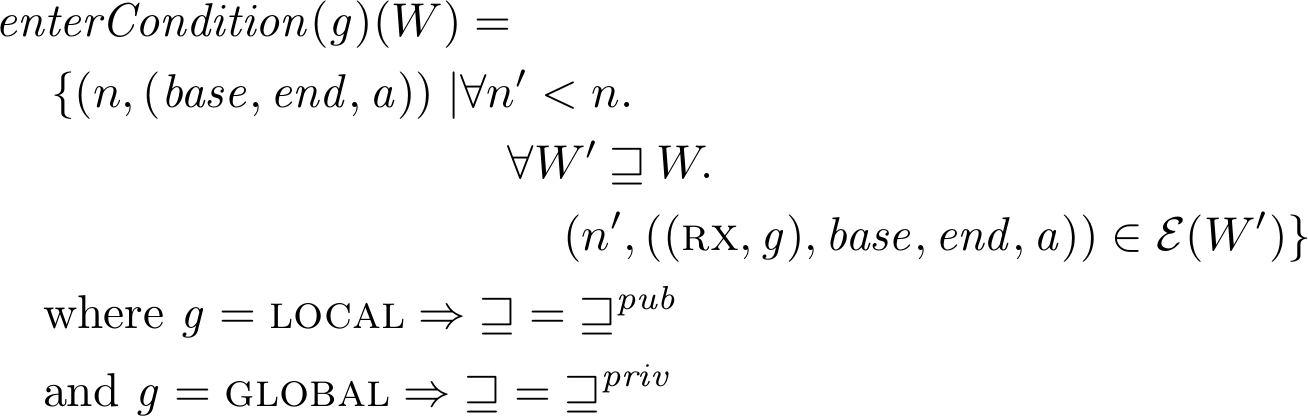
\includegraphics[width=\textwidth]{econd}
\end{frame}

\begin{frame}
  \frametitle{Flavours of linear capabilities}
  \begin{columns}
\begin{column}{.7\textwidth}
  \begin{itemize}
  \item unique linear capability\\
    \begin{itemize}
    \item No alias
    \item \stktokens{}-paper
  \end{itemize}
\item linear\\
  \begin{itemize}
  \item May have aliases
  \item CHERI
  \end{itemize}
  \end{itemize}
\end{column}
\begin{column}{.3\textwidth}
  \begin{tikzpicture}
    \node (ul) {unique linear};
    \node[below=of ul] (n) {normal};
    \node[below=of n] (l) {linear};
    \draw (ul) -- (n) -- (l);
  \end{tikzpicture}
\end{column}
\end{columns}
\end{frame}

\end{document}

% \begin{frame}<1-2>[label=machine]
% %  \frametitle{Machine}
%   \begin{columns}
%     \begin{column}{.6\textwidth}
%       \begin{tikzpicture}[scale=.45, every node={scale=.5}]
%         \scope
%           \clip (-.1,-.1) rectangle (6.1,14.9);
%           \fill[draw,fill=white] (0,0) rectangle (6,15);
%         \endscope
%         % \draw[->] (-2,0) -- node[midway,sloped,above] {stack grows upward}
%         % (-2,15);
%         \foreach \X in {0,0.5,...,14} {
%           \fill[draw,fill=white] (0,\X) rectangle (6,\X+.5) node[pos=.5] { };
%         };
%         \draw (-0.6,-0.1) node[rotate=45, align=right] { \scriptsize\texttt{0x00} };
%         \draw (-0.6,3.9)  node[rotate=45, align=right] { \scriptsize\texttt{0x08} };
%         \draw (-0.6,7.9)  node[rotate=45, align=right] { \scriptsize\texttt{0x10} };
%         \draw (-0.6,11.9) node[rotate=45, align=right] { \scriptsize\texttt{0x16} };

%   \begin{scope}
%     \clip (9.9,2.6) rectangle (11.6,11.6);
%     \foreach \X in {0,1.5,...,7.5} {
%       \fill[draw,fill=white] (10,10 - \X) rectangle (11.5,11.5-\X) node[pos=.5] { };
%     };
%   \end{scope}
%   \draw (10.75,12.25) node[align=center] {Register File};
%   \draw (6.5,14.325) node[anchor=west, align=left] {Memory};

%   % Mem data
%   \draw<1-> (3,0.75) node { \scriptsize\texttt{0x2a}};
%   \draw<1-> (3,1.25) node { \scriptsize\texttt{0x02}};
%   \draw<1-> (3,1.75) node { \scriptsize\texttt{0x0e}};
%   \draw<1-> (3,2.75) node { \scriptsize\texttt{0x0a}};
%   \draw<1-> (3,2.25) node { \scriptsize\texttt{0x13}};
%   \draw<1-> (3,3.75) node { \scriptsize\texttt{0x00}};
%   \draw<1-> (3,3.25) node { \scriptsize\texttt{0x00}};
%   \draw<1-> (3,4.25) node { \scriptsize\texttt{0x00}};
%   \draw<1-> (3,4.75) node { \scriptsize\texttt{0x00}};
%   \draw<1-> (3,5.75) node { \scriptsize\texttt{0x03}};
%   \draw<1-> (3,6.25) node { \scriptsize\texttt{0x14}};
%   \draw<1-> (3,6.75) node { \scriptsize\texttt{0x15}};
%   \draw<1-> (3,7.25) node { \scriptsize\texttt{0x0b}};
%   \draw<1-> (3,7.75) node { \scriptsize\texttt{0x0a}};
%   \draw<1-> (3,8.25) node { \scriptsize\texttt{0x0f}};
%   \draw<1-> (3,8.75) node { \scriptsize\texttt{0x13}};
%   \draw<1-> (3,9.25) node { \scriptsize\texttt{0x1b}};
%   \draw<1-> (3,9.75) node { \scriptsize\texttt{0x00}};
%   \draw<1-> (3,10.25) node { \scriptsize\texttt{0x00}};
%   \draw<1-> (3,10.75) node { \scriptsize\texttt{0x00}};
%   \draw<1-> (3,11.25) node { \scriptsize\texttt{0x00}};
%   \draw<1-> (3,11.75) node { \scriptsize\texttt{0x00}};
%   \draw<1-> (3,12.75) node { \scriptsize\texttt{0x00}};
%   \draw<1-> (3,13.25) node { \scriptsize\texttt{0x00}};
%   \draw<1-> (3,13.75) node { \scriptsize\texttt{0x40}};
%   \draw<1-> (3,14.25) node { \scriptsize\texttt{0x05}};
%   % Reg data
%   \draw<1-> (10.75,10.75) node { \scriptsize\texttt{0x08}};
%   \draw<1-> (10.75,7.75) node { \scriptsize\texttt{0x18}};
%   \draw<1-> (10.75,6.25) node { \scriptsize\texttt{0x10}};
%   \draw<1-> (10.75,4.75) node { \scriptsize\texttt{0x02}};

%   % Mem pointers
%   \draw<1> (3,12.25) node { \scriptsize\texttt{0x10}};
%   \draw<1> (3,5.25) node { \scriptsize\texttt{0x0b}};
%   \draw<1> (3,0.25) node { \scriptsize\texttt{0x08}};
%   % Reg pointers
%   \draw<1> (10.75,9.25) node { \scriptsize\texttt{0x00}};

%   % Mem pointers HL
%   \draw<2> (3,12.25) node { \color{red} \scriptsize\texttt{0x10}};
%   \draw<2> (3,5.25) node { \color{red} \scriptsize\texttt{0x0b}};
%   \draw<2> (3,0.25) node { \color{red} \scriptsize\texttt{0x08}};
%   % Reg pointers HL
%   \draw<2> (10.75,9.25) node { \color{red} \scriptsize\texttt{0x00}};

%   \draw<3> (10.75,9.25) node { };

%   % Mem capabilities
%   \draw<4->[capa] (3,12.25) edge[postaction={decorate}] (6.1,12.25 );
%   \draw<4> (6.1,12.25) edge[-latex,in=0,out=0] (6.1,8.25);
%   \draw<4->[capa] (3,5.25) edge[postaction={decorate}] (6.1,5.25);
%   \draw<4> (6.1,5.25) edge[-latex,in=0,out=0] (6.1,6.75);
%   \draw<4->[capa] (3,0.25) edge[postaction={decorate}] (6.1,0.25);
%   \draw<4> (6.1,0.25) edge[-latex,in=0,out=0] (6.1,4.25);

%   % Reg pointers HL
%   \draw<4->[capa] (10.75,9.25) edge[postaction={decorate}] (10.5,9.25);
%   \draw<4> (10.5 ,9.25) edge[-latex,in=0,out=180] (6.1,0.25);

%   % Mem capabilities \w auth
%   \draw<5> (6.1,12.25) edge[-latex,in=0,out=0] (6.5,8.25);
%   \draw<5->[decorate,decoration={brace,amplitude=2pt,raise=0pt,aspect=0.55,mirror},yshift=0pt] (6.3,5.5) -- (6.3,10.5) node (e) [black,midway,xshift=0.8cm] {};

%   \draw<5> (6.1,5.25) edge[-latex,in=0,out=0] (6.3,6.75);
%   \draw<5-> [decorate,decoration={brace,amplitude=2pt,raise=0pt,aspect=0.5,mirror},yshift=0pt] (6.1,6) -- (6.1,7.5) node (e) [black,midway,xshift=0.8cm] {};


%   \draw<5> (6.1,0.25) edge[-latex,in=0,out=0] (6.5,4.25);
%   \draw<5-> [decorate,decoration={brace,amplitude=2pt,raise=0pt,aspect=0.5,mirror},yshift=0pt] (6.3,3) -- (6.3,5.5) node (e) [black,midway,xshift=0.8cm] {};


%   % Reg pointers HL \w auth
%   \draw<5> (10.5,9.25) edge[-latex,in=0,out=180] (6.3,0.355);
%   \draw<5-> [decorate,decoration={brace,amplitude=2pt,raise=0pt,aspect=0.1,mirror},yshift=0pt] (6.1,0) -- (6.1,3.5) node (e) [black,midway,xshift=0.8cm] {};

%   % Mem capabilities \w auth & perm
%   \draw<6-> (6.1,12.25) edge[-latex,in=0,out=0] node[right] {\scriptsize \textsc{r}} (6.5,8.25);

%   \draw<6-> (6.1,5.25) edge[-latex,in=0,out=0] node[right] {\scriptsize \textsc{rw}} (6.3,6.75);

%   \draw<6-> (6.1,0.25) edge[-latex,in=0,out=0] node[right] {\scriptsize \textsc{r}} (6.5,4.25);

%   % Reg pointers HL \w auth & perm
%   \draw<6-> (10.5,9.25) edge[-latex,in=0,out=180] node[right] {\scriptsize \textsc{rx}} (6.3,0.355);
% \end{tikzpicture}
% \end{column}
% \begin{column}{0.4\textwidth}
%   \onslide<3->{Replace pointers with capabilities}
%   \begin{itemize}
% nnn  \item<4-> Pointer
%   \item<5-> Range of authority
%   \item<6-> Permission
%   \end{itemize}
%   \onslide<7->{Dynamically enforced}
%   \begin{itemize}
%   \item<8-> Cap. aware instructions
%   \item<9-> Tagged memory
%   \end{itemize}
% \end{column}
% \end{columns}
% \end{frame}
